\documentclass[linenumbers,draft]{agujournal}
\journalname{Space Weather}

% Create numbered lines
%\usepackage{lineno}
%\linenumbers*[1]

%  To add line numbers to lines with equations:
%  \begin{linenomath*}
%  \begin{equation}
%  \end{equation}
%  \end{linenomath*}

%  Include .eps files
%\usepackage{graphicx}
% Table problem
%\usepackage{morefloats}
% Color tables
%\usepackage[table]{xcolor}
% Multirow package
\usepackage{multirow}
% Multipage table
\usepackage{longtable}

% Colors
\definecolor{Red}{rgb}{1,0,0}

%  Allow illustrations to print when using Draft:
\setkeys{Gin}{draft=false}

% Author names in capital letters:
%\authorrunninghead{FACSK{\'O} ET. Al.}

%\renewcommand{\arraystretch}{0.6}

\begin{document}


\title{Comparing 1-year GUMICS$-$4 simulations of the Terrestrial Magnetosphere with Cluster Measurements}

\authors{G.~Facsk{\'o}\affil{1,2,3}\thanks{Now at Rhea System GmbH, TIZ Building, Robert Bosch Str. 7, 64293 Darmstadt, Germany}, D.~G.~Sibeck\affil{2}, I.~Honkonen\affil{4}, L.~Degener\affil{4}\thanks{Now private individual, Hannover, Germany}, P.~Peitso\affil{5}\thanks{Now at Aurora Propulsion Technologies, Espoo, Finland }, E.~I.~Tanskanen\affil{5}, C.~R.~Anekallu\affil{6}, J.~Kalm{\'a}r\affil{1}, J.~B{\'o}r\affil{1}, G.~Farinas~Perez\affil{2,3}\thanks{Now at University of Miami, Electrical and Computer Engenieering Department, Miami, Florida, USA}, S.~Szalai\affil{1}, {\'A.}~Kis\affil{1}, V.~Wesztergom\affil{1}} % Y.~Y.~Shprits\affil{8,9}, N.~A.~Aseev\affil{8,9}

\affiliation{1}{HAS Research Centre for Astronomy and Earth Sciences, Sopron, Hungary}
\affiliation{2}{NASA Goddard Space Flight Center, Greenbelt, Maryland, USA}
\affiliation{3}{the Catholic University of America, Washington DC, USA}
\affiliation{4}{Finnish Meteorological Institute, Helsinki, Finland}
\affiliation{5}{Aalto University, School of Electrical Engineering, Espoo, Finland}
\affiliation{6}{UCL Department of Space \& Climate Physics, Mullard Space Science Laboratory, Dorking, UK}
%\affiliation{7}{Helmholtz Centre Potsdam, GFZ German Research Centre for Geosciences, Potsdam, Germany}
%\affiliation{8}{Institute for Physics and Astronomy, University of Potsdam, Potsdam, Germany}

\correspondingauthor{G{\'a}bor Facsk{\'o}}{gabor.i.facsko@gmail.com}
% German: gxf261@miami.edu

\begin{keypoints}
\item The GUMICS$-$4 provides realistic ion plasma moments and magnetic field in the solar wind and the outer magnetosheath.
\item The code can provide the realistic location of the bow shock.
\item An inner magnetosphere model should add to the code to increase the accuracy of the simulation.
\end{keypoints}

\begin{abstract}
Previously 1-year global magnetohydrodynamics simulation was made using the GUMICS$-$4 code and the OMNI 1-min resolution solar wind data from January 29, 2002 to February 2, 2003 as input. Along the orbit of the Cluster SC3 reference spacecraft the simulation data was saved. We compare the saved parameters to the Cluster SC3 measurements. We use the magnetic field Z component, the solar wind velocity X component and the solar wind density of the Cluster magnetometer, ion plasma and spacecraft potential measurements geocentric solar ecliptic reference frame. We select intervals in the solar wind, the magnetosheath and the magnetosphere where the instruments above provided good quality data and the spacecraft and the simulation are in the same region. We determine the location of the bow shock, the magnetopause and the neutral sheet in the spacecraft measurements and compare their position in the observation and simulations.

The GUMICS$-$4 provides quite good results in the solar wind. Its accuracy is significantly worse in the magnetosheath. The simulation results are not realistic in the magnetosphere. The bow shock location is predicted well however the magnetopause location is less accurate. The neutral sheet positions are located quite well thank to the special solar wind conditions. The reason of these inaccuracies is the missing inner magnetosphere model and the obsolete algorithms applied in the code.
\end{abstract}


\section{Introduction}
\label{sec:introduction}

The most cost-effective way to study the interaction of the solar wind and the planetary magnetospheres (or predict the conditions of the near-Earth space) is using a global magnetohydrodynamics (MHD) code. Robust parallelized, effective, verified and validated codes were developed, are used and applied to forecast the cosmic environment of the Earth; such as the Lyon-Fedder-Mobarry, LFM \citep{lyon04:_lyon_fedder_mobar_lfm_mhd} code, the Open Geospace General Circulation Model, OpenGGCM \citep{raeder08:_openg_simul_themis_mission}, the Block-Adaptive-Tree-Solarwind-Roe-Upwind-Scheme, BATS-R-US \citep{powell99:_solut_adapt_upwin_schem_ideal_magnet,toth12:_adapt}. In Europe only three global MHD codes were developed: the Grand Unified Magnetosphere--Ionosphere Coupling Simulation \citep[GUMICS$-$4;][]{janhunen12:_gumic_mhd}, the COOLFluiD \citep{lani12:_coolf_open_comput_platf_aerot} and the GORGON 3D magnetohydrodynamic code. The COOLFluiD is a general-purpose plasma simulation tool. The Gorgon code was developed for studying high energy, collisional plasma interactions and has been adapted to simulate planetary magnetospheres and their interaction with the solar wind \citep{mejnertsen16:_global_mhd_neptun,mejnertsen18:_global_mhd_simul_earth_bow}. The GUMICS$-$4 was developed to study the solar wind-terrestrial magnetosphere interaction and its paralel version has not been available for the scientific community (see Section~\ref{sec:gumics}). These codes are available at the Community Coordinated Modelling Center (CCMC; http://ccmc.gsfc.nasa.gov/) hosted by the NASA Goddard Space Flight Center (GSFC). The comparison of the simulation results to spacecraft and ground-based measurements is necessary to understand the abilities and features of the developed tools. The statistical study using long term global MHD runs for validation and verification of the codes seems to be a good and fruitful method. However, providing long simulations is costly and time consuming hence only a few study had done previously using much shorter simulations than a year. 

\citet{guild08:_geotail_lfm1,guild08:_geotail_lfm2} launched two months of LFM run and compared the plasma sheets properties in the simulated tail to the statistical properties of six years Geotail magnetic field and plasma observations \citep{kokubun94:_geotail_magnet_field_exper,mukai94:_low_energ_partic_lep_exper_geotail_satel}. The LFM successfully reproduced the global features of the global plasma sheet in statistical sense. However, there were some differences. The sheet was too cold, too dense and the bulk flow was faster than the observed plasma sheet. The LFM overestimated the ionospheric transpolar potential. The transpolar potential correlated with the speed of the plasma sheet flows. The equatorial maps of density, thermal pressure, thermal energy and velocity were compared. The LFM overestimated the plasma sheet density close to the Earth and underestimated the temperature by a factor of $\sim$3. The LFM overestimated the global average flow speed by a factor of $\sim$2. The LFM reproduced many of the climatological features of the Geotail data set. The low-resolution model underestimated the occurrence of the fast earthward and tailward flows. Increasing the simulation resolution resulted the development of fast, busty flows. These flows contributed the statistics and brought closer the simulations to the observations.

\citet{zhang11:_lyon_fedder_mobar_mhd} launched two months long LFM simulation to study the statistics of magnetosphere-ionosphere (MI) coupling. The LFM simulation was also used in the previous study of \citet{guild08:_geotail_lfm1}. The polar cap potential and the field aligned currents (FAC), the downward Poynting flux and the vorticity of the ionospheric convection were compared with observed statistical averages and the Weimer05 empirical model \citep{weimer05:_improv_joule}. The comparisons showed that the LFM model produced quite accurate average distributions of the Region 1 (R1) and Region 2 (R2) currents. The ionospheric Region 2 currents in the MHD simulation seemed to be originated from the diamagnetic ring current. The average LFM Region 1 and 2 currents were smaller compared with the values from the Weimer05 model. The average CPCP was higher in the LFM simulation than the measurements of the SuperDARN and the Weimer05 model. The average convention pattern was quite symmetric in the LFM simulation against the SuperDARN measurements and the Weimer05 model. The SuperDARN measurements and the Weimer05 model had dawn-dusk asymmetry. In the LFM, model more Poyting flux flowed into the polar region ionosphere than in the Weimer05 model. It was the consequence of the larger CPCP in the LFM simulation. The larger CPCP allowed higher electric field in the polar region. The statistical dependence of the high-latitude convection patterns on Interplanetary Magnetic Field (IMF) clock angle was similar to the SuperDARN measurements \citep{sofko95:_direc_super} and the Weimer05 model. The average ionospheric field-aligned vorticity showed good agreement on the dayside. However, the LFM model gave larger nightside vorticity than SuperDARN measurements because the Pedersen conductance on the night side ionosphere was too low. 

\citet{wiltberger17:_struc_high_latit_curren_magnet_ionos_model} studied the structure of the high latitude field-aligned current patterns using three resolutions of the LFM global MHD code and the Weimer05 empirical model \citep{weimer05:_improv_joule}. The studied period was a month long and contained two high-speed streams. Generally, the patterns agreed well with results obtained from the Weiner05 computing. As the resolution of the simulations increased, the currents became more intense and narrow. The ratio of the Region 1 (R1), the Region 2 (R2) currents and the R1/R2 ratio increased when the simulation resolution increases. However, both the R1 and R2 currents were smaller than the predictions of the Weimer05 model. This effect led better agreement of the LFM simulation results to the Weimer~2005 model results. The CPCP pattern became concentrated in higher latitudes because of the stronger R2 currents. The relationship of the CPCP and the R1 looked evident at higher resolution of the simulation. The LFM simulation could have reproduced the statistical features of the field aligned current (FAC) patterns. 

\citet{haiducek17:_swmf_global_magnet_simul_januar} simulated a month of January 2005 using the Space Weather Modelling Framework \citep[SWMF;][]{toth05:_space_weath_model_framew} and the OMNI solar wind data as input. The simulations were done with and without inner magnetosphere model and using two different grid resolutions. The model was very good in predicting the currents circling the Earth around the dipole axis \citep[SYM-H; http://wdc.kugi.kyoto-u.ac.jp/aeasy/asy.pdf;][]{iyemori90:_storm}. The $K_p$ index (that measures the general magnetospheric convention and the auroral currents \citep{bartels39,rostoker72:_geomag,thomsen04:_why_kp}) was predicted well during storms however the index was over predicted during quiet time periods. The AL index (that describe the westward electro jet on the surface magnetic field introduced by \citet{davis66:_auror_ae}) was predicted reasonably well in average however the model reached the highest negative AL value less often than the observations because the model captured poorly the structure of the auroral zone currents. The overpredicting of $K_p$ index during quiet times might have had the same reason because that index was also sensitive for the auroral zone dynamics. The SWMF usually over predicted the CPCP. These results were not sensitive to grid resolutions. Except that the AL index reached more often the highest negative value when the grid resolution was higher. Switching off of the inner magnetosphere model had dramatic effect for the accuracy of all quantities mentioned above, except the CPCP. 

In this paper the Cluster SC3 measurements are compared directly to a previously made 1-year long GUMICS$-$4 simulation in the solar wind, magnetosheath and the magnetosphere along the Cluster SC3 orbit saved from the simulation results and measured by the spacecraft \citep{facsko16:_one_earth}. Three parameters ($B_z$, $V_X$ and $n$) were studied and the location of the bow shock, magnetopause and the neutral sheet. The structure of this paper is as follows. Section~\ref{sec:data} describes the GUMICS$-$4 code, the 1-year simulation and the instruments. Section~\ref{sec:comp} gives comparisons between the simulations and observations. Results of the comparison are discussed in Section~\ref{sec:discussion}. Finally, Section~\ref{sec:concl} contains the conclusions.

\section{The GUMICS$-$4 products and Cluster measurements}
\label{sec:data}

Here we use two types of very different and difficult time series. The first type is derived from previously made 1-year GUMICS$-$4 simulation \citep{facsko16:_one_earth}. The second type was measured by the magnetometer, ion plasma and electric field instruments of the Cluster reference spacecraft.

\subsection{The GUMICS$-$4 code}
\label{sec:gumics}

The GUMICS$-$4 has two coupled simulation domains, the magnetospheric domain outside of 3.7\,$R_E$ radius around the Earth and a coupled ionosphere module containing a 3D electron density model if the ionosphere. The GUMICS$-$4 is not parallel code however the code was extensively used for studying the energy propagation processes from the solar wind to the magnetosphere through the magnetopause and other features \citep[][see the references therein]{janhunen12:_gumic_mhd}. The code had also been applied for study the forced reconnection in the tail \citep{voeroes14:_winds_condit_ram_co_ram}. Recently a few hundred of synthetic two hours duration GUMICS$-$4 simulations was made to compare the simulation results to empirical formulas \citep{gordeev13:_verif_gumic_mhd}. The agreement was quite good however; the diameter of the magnetopause deviated significantly in the simulation and the observations in the tail. The tail of the GUMICS$-$4 was smaller than spacecraft observed and measured. 1-year long simulation was made using the GUMICS$-$4 code \citep{facsko16:_one_earth}. \citet{juusola14:_statis_gumic_mhd} compared the ionospheric currents, fields and the cross polar cap potential (CPCP) in the simulation versus Super Dual Auroral Radar Network (SuperDARN) radars \citep{greenwald95:_darn_super} and CHAMP spacecraft \citep{reigber02:_champ} field aligned currents (FAC) measurements \citep{juusola07:_hall_peder_champ,ritter04:_ionos_champ_image}. The agreement was good the seasonal variation of the CPCP however the FAC and other currents could not be reproduced properly. The possible reason of this bad agreement could be the leak of the inner magnetosphere model. This statement is supported by the result of \citet{haiducek17:_swmf_global_magnet_simul_januar}. \citeauthor{haiducek17:_swmf_global_magnet_simul_januar} simulated only a month using different spatial resolution and to test the codes switched off the inner magnetosphere model of the SWMF for a special run.  This run without inner magnetosphere model resulted that only the CPCP parameter of the simulation agreed quite well with the measurement. This fact explained why was so good the agreement between the Cluster SC3 and the GUMICS$-$4 simulations and gave sense to provide the studies of \citet{lakka18:_cross_polar_cap_satur_gumic,lakka18:_icme_earth_mach} based on the CPCP in GUMICS$-$4 simulations. \citet{kallio15:_proper} determined the solar wind parameters along the Moon orbit using the results of the \citet{facsko16:_one_earth}'s global MHD simulations. The solar wind parameters differed significantly in the geotail that should have been considered in future studies of the interaction of the solar wind and the lunar orbit. \citet{facsko16:_one_earth} determined the footprint the Cluster SC3 using the 1-year simulation and the Tsyganenko T96 empirical model \citep{tsyganenko95:_model_earth}. The code seemed to be react slower for the dynamic changes of the solar wind pressure than the empirical model. The agreement of the footprint is better in the Northern Hemisphere. The GUMICS$-$4 tail looked shorter in the simulations than the observations. Finally, the Y component of the interplanetary magnetic field twisted the simulated tail hence the agreement of the empirical and computational footprints was worse at such solar wind conditions.

A workpackage of the European Cluster Assimilation Technology (ECLAT) project (https://cordis.europa.eu/result/rcn/165813\_en.html; http://www.eclat--project.eu/) was the creation and analysis of 1-year global MHD simulation using the OMNI solar wind data  from January 29, 2002 to February 2, 2003 as input of the GUMICS$-$4 code \citep{facsko16:_one_earth}. The GUMICS-4 was a single core system \citep{janhunen12:_gumic_mhd} hence the 1-year simulation was made in 1860 independent runs. This interval covered 155 Cluster SC3 orbits and each orbit lasted 57 hours. The supercomputer had 12 CPUs on each node hence the 57 hours were divided into 4.7 hours simulation time with one hour initialisation period. Each sub-intervals used its own average Geocentric Solar Ecliptic (GSE) IMF magnetic field X component $B_x$ component and dipole tilt angle. All data gaps of the input file were filled using interpolation. If the data gap of the input file was at the beginning (or the end) interval the first (or last) good data of the input file was used to fill the gap. The initialisation of each simulations was made using constant values. These values were the first valid data of the input file repeated 60 times (60 minutes) in the input file of the sub-interval. The simulation results were saved in every five minutes. Various simulation parameters, for example, the density, particle density, temperature, magnetic field, solar wind velocity (29 different quantities) were saved from the simulation results along the Cluster reference spacecraft in the GSE coordinates. In this paper these parameters, namely the $B_z$ magnetic field GSE Z component, the solar wind velocity GSE X component ($V_x$) and the solar wind density $n$ are compared to the Cluster SC3 measurement. These parameters are selected because the $B_z$ controls the magnetosphere, the $V_x$ is the main solar wind velocity component and the $n$ is the ion plasma momentum that is the easiest to calculate; furthermore more instruments could determine it (see Section~\ref{sec:cluster}).

\subsection{The Cluster SC3 measurements}
\label{sec:cluster}

The Cluster-II spacecraft of the European Space Agency (ESA) were launched in 2000 and study the geospace since then \citep{credland97:_clust_mission,escoubet01:_introd_clust}. Its four spacecraft form a tetrahendron however here we use only the measurements of the reference spacecraft, the Cluster SC3. The spacecraft were stabilised by rotation and its period is $\sim$4\,s. Hence, the temporal resolution of the plasma instruments were considered 4\,s and we use 4\,s averaged magnetic field data. The real resolution of the Cluster FluxGate Magnetometer (FGM) magnetic field instrument was 27\,Hz \citep{balogh97:_clust_magnet_field_inves,balogh01:_clust_magnet_field_inves}. The ion plasma data was provided by the Cluster Ion Spectrometry (CIS) Hot Ion Analyser (HIA) sub-instrument \citep{reme97:_clust_ion_spect_exper,reme01:_first_earth_clust_cis}. The CIS HIA instrument is calibrated using the Waves of HIgh frequency Sounder for Probing the Electron density by Relaxation (WHISPER) wave instrument onboard Cluster \citep{decreau01:_early_whisp_clust,trotignon10:_whisp_relax_sound_clust_activ_archiv,blagau13:_in_hot_ion_analy_clust,blagau14:_in_hot_ion_analy_clust}. These calibrations might have appeared as sudden non-physical jumps in the CIS HIA data. The CIS HIA had different modes to measure in the solar wind and the magnetosphere. When the instrument switched from a mode to another mode it appeared as a non-physical jump in the measured data too. These features had influence for the accuracy of the data analysis.

We protect our results from these non-physical jumps described previously using a density determination based on different principles. We use the spacecraft potential of the Electric Field and Wave Experiment \citep[EFW ;][]{gustafsson97:_elect_field_wave_exper_clust_mission,gustafsson01:_first_clust_efw} to determine the electron density. This quantity can be calculated using the empirical density formula 
\begin{equation}\label{eq:empdens}
n_{EFW}=200(V_{sc})^{-1.85},
\end{equation}
where $n_{EFW}$ is the calculated density and $V_{sc}$ is the Cluster EFW spacecraft potential \citep{trotignon10:_whisp_relax_sound_clust_activ_archiv,trotignon11:_calib_repor_whisp_measur_clust}. The EFW and the WHISPER were used for the calibration of the CIS HIA and the Plasma Electron and Current Experiment \citep[PEACE;][]{johnstone97:_peace,fazakerley10:_peace_data_clust_activ_archiv,fazakerley10:_clust_peace_in_calib_status}. Both instruments were still working onboard all Cluster spacecraft. Their stable operation reduced the number of data gaps; furthermore made easier the data analysis.

\section{Comparison of measurements to simulation}
\label{sec:comp}

The saved parameters from the GUMICS$-$4 simulations and the Cluster SC3 magnetic field, solar wind velocity and density measurements are compared in the solar wind, magnetosheath and magnetosphere using cross correlation calculation. The resolution of the simulated Cluster orbit data is mostly five minutes because the simulations are saved in every five minutes \citep{facsko16:_one_earth}. However, the time difference between points could be more than five minutes at the boundary of the subintervals, because the length of simulation intervals is determined in minutes. To facilitate analysis of the simulation results, all simulation data were interpolated to one minute resolution. This method does not provide extra information to the cross correlation calculation. The data gaps are eliminated using interpolation in the data and extrapolation when the gap is at the start or the end of the selected interval. The spin resolution (4\,s) of Cluster SC3 magnetic field measurements is averaged over one minute around ($\pm30\,s$) the time stamps of the saved data. 

For the correlation calculation intervals are selected carefully in the solar wind, the magnetosheath, the dayside and the night side magnetosphere. In these intervals the parameters do not varied a lot and neither the Cluster nor the virtual probe crossed any boundary layer. To compare the shape of the $B_z$ magnetic field, $V_x$ solar wind speed and the $n_{CIS}$ and the $n_{EFW}$ curves we calculate cross correlation on selected intervals. Sometimes we get very bad results. Then we examined carefully the case and removed the short intervals (shorter than four hours) from the correlation calculation and large data gaps from the correlation calculation. (The data gaps are interpolated however they cause loss of information.) Those intervals are also neglected where the plasma instrument has calibration error or changed its mode from magnetosphere to solar wind (for example). The electron density is also calculated using the empirical density formula (see Equation~\ref{eq:empdens}) and make the correlation calculation. We want to avoid calibration errors and sudden non-physical jumps mentioned previously. The results do not differ significantly however the $n_{EFW}$ has not mode change and it is applicable in the magnetosphere too (against the CIS HIA instrument).

\subsection{Solar wind}
\label{sec:sw}

We use OMNI IMF and solar wind velocity, density and temperature data as input of the simulation. However, it is not useless to compare the solar wind region in the simulation and the measurements. The IMF X component cannot be given to the GUMICS$-$4 as input \citep{janhunen12:_gumic_mhd,facsko16:_one_earth}. However the magnetic field of the solar wind has X component in the simulations. Additionally the solar wind structure might change from the simulation domain boundary at +32\,$R_E$ to the sub-solar point of the terrestrial bow shock where all OMNI data is shifted. Almost the same solar wind intervals are used as in the see Table~1 of \citet{facsko16:_one_earth}. The number of these intervals is small because the Cluster fleet instruments were calibrated in 2002, just after launching (Table~\ref{tab:sw}). Hence we do not have so good ion plasma data coverage for this year. Additionally, to improve the accuracy of the correlation calculation (see below) we delete those intervals which were too short (shorter than five hours) or the CIS HIA instrument changed its mode. The Cluster fleet is located in the solar wind only from December to May and only for a couple of hours during each orbit near to the apogee. We double check whether the Cluster SC3 stays in the solar wind in both the simulation and the reality. We also check the omnidirectional CIS HIA ion spectra on the Cluster Science Archive (CSA; https://www.cosmos.esa.int/web/csa/csds-quicklook-plots). Hence 17 intervals are remained in the solar wind to study (Figure~\ref{fig:sworbit}). 

The selected intervals have quiet solar wind conditions (Figure~\ref{fig:swomni}). The GUMICS$-$4 simulation results have five minutes resolution and the Cluster SC3 measurements have one minutes resolution (Figure~\ref{fig:swplot}). The measurements vary significantly. Inspect of the quiet conditions the solar wind density often changes and deviates from the simulation. On the left of the Figure~\ref{fig:swscatplot} both densities deviate significantly. The CIS HIA density deviation is larger as it is expected because of the complexity and the large number of working modes of the CIS instrument. The magnetic field and the solar wind velocity fit better. On the left side of the Figure~\ref{fig:swcorrplot} the correlation of the magnetic field is very good; furthermore the correlation of the solar wind velocity and density is excellent (Table~\ref{tab:sw}). The time shift on the right side of the Figure~\ref{fig:swcorrplot} is about five minutes for the magnetic field and the CIS data. For the EFW data the time shift is worse. It is not determined as well as the other parameters.

\subsection{Magnetosheath}
\label{sec:msh}

The Cluster SC3 spent only a few time in the solar wind from December, 2002 to May, 2003. However, the orbit of the spacecraft always crosses the magnetosheath (Figure~\ref{fig:mshorbit}). We selected intervals when the value of the magnetic field is around 25\,nT. The field should be fluctuating because of the turbulent and deviated flow of the solar wind after passing the bow shock. In the same time the solar wind temperature increases. The solar wind speed drops it value is only 100-300\,km/s. The density of the plasma flow increased and reached the 10-20\,cm\textsuperscript{-3}.  The narrow band on the  omnidirectional CIS HIA ion spectra from the CSA (https://www.cosmos.esa.int/web/csa/csds-quicklook-plots) is widened after passing the bow shock. After 15-30 \,min this passage we considered the Cluster SC3 to be entered to the magnetosheath. At the inner boundary the flow speed drops and the density as well. The magnetic field starts growing and it is less turbulent than in the magnetosheath. The wide band on the  the omnidirectional CIS HIA ion spectra disappears. 15-30 minutes before the appearance  of these indicators of the magnetopause crossing our intervals end. All intervals contain large data gap, non-physical jump of instrument mode changing or shorter than four hour are removed. Hence 74 intervals considered in our final selection (Table~\ref{tab:msh}). 

All intervals have quiet upstream (or input) solar wind conditions (Figure~\ref{fig:mshomni}). Inspect of our selection the magnetic field and the plasma parameters and the calculated empirical density vary significantly stronger than in the solar wind intervals (Figure~\ref{fig:mshplot}). The deviation of the simulated and the observed data is larger in this region as well. The scattered plots of the magnetic field, plasma flow speed and the densities agree well however these plot relatively less accurate than the scattered plots of the solar wind (Figure~\ref{fig:mshscatplot}). The correlation of the simulated and the observed data is good for the magnetic field, very good for the ion plasma moments and the calculated density (Figure~\ref{fig:mshcorrplot}, left). The timeshift of the magnetic field is within five minutes mostly however the timeshift of the ion plasma moments is scattered. The timeshift of the calculated EFW density seems to be more accurate. Generally, the GUMICS$-$4 is less accurate in the magnetosheath. The magnetic field is quite good however the plasma parameters are not so good. The calculated empirical EFW density ($n_{EFW}$) fits better than the CIS HIA density ($n_{CIS}$).


\subsection{Magnetosphere}
\label{sec:msph}

To select intervals in the magnetosphere we looked for the CIS HIA OMNI directional ionflux. When the band of the hot magnetosheath ion population (dis)apperared, the magnetosphere started/finished. The solar wind density becomes slowly zero, a magnetic field and the solar wind density drop and reach the zero value. We left 15-30\,min after/before the magnetopause transition to appoint the interval in the magnetopshere. In this way we found 132 intervals in the magnetosphere (Table~\ref{tab:msph}) using Cluster SC3 measurements. The Cluster SC3 spends considerable time in the magnetosphere (Figure~\ref{fig:msphorbit}). 

Here we show neither any correlation calculation nor comparison plot. In the magnetosphere the GUMICS$-$4 does not work well. Neither the magnetic field nor the plasma moments nor the $N_{EFW}$ fit well. The solar wind velocity does not reach zero in the simulation. Instead the solar wind enters to the night side magnetosphere. The solar wind CIS HIA ion plasma density and the calculated density from spacecraft potential increase closer to the Earth (plasmasphere). The GUMICS$-$4 density is low there. We calculated the dipole field in GSE using Tsyganenko geotool box \citep{tsyganenko95:_model_earth} and subtracked from both the observed and the simulated magnetic field $B_z$ data. The correlation of these corrected magnetic field measurements and simulations is very low too. 

\subsection{Bow shock, magnetopause, neutral sheet}
\label{sec:bs}

78 intervals are selected when the Cluster SC3 crossed the terrestrial bow shock once or multiple times. When the spacecraft crosses the bow shock inward direction the magnitude of the magnetic field and the solar wind density increases 4-5 times (from 5\,nT or 5\,$cm^{-3}$, respectively), the solar wind speed drops from 400--600\,km/s to 100--300\,km/s; furthermore the narrow band on the omnidirectional Cluster CIS HIA ion spectra is widened. The Cluster measurements are 1-min averaged and the GUMICS$-$4 simulations has 5-min resolution hence all bow shock transitions of the virtual spacecraft are slower and smoother. Additionally, the multiple bow shock transitions are not visible in the $\mathrm{GUMICS}$ simulations. The code reacts slowly for such sudden changes. The magnetic signatures fit better than the calculated plasma moments. The jump of the ion plasma parameters and the derived Cluster EFW density of the simulations are shifted to the measurements. Generally, the density and the velocity of the simulations seem to be less accurate than the magnetic field of the simulations.

56 intervals are selected around magnetopause crossings (Anekallu, private communication). When the spacecraft crosses the magnetopause inward direction the magnitude of the magnetic field increases, the solar wind speed drops from 100--300\,km/s to zero, the plasma density becomes zero; furthermore the wide band on the omnidirectional Cluster CIS HIA ion spectra disappears. These changes are not so fast. The location of the magnetopause is well determined by the Cluster SC3 measurements. However, it is very difficult to identify the magnetopause crossings in the simulation data. The 5-min resolution of the simulations provides smooth and averaged curves without sharp changes. Furthermore, the magnetopause crossings very often cannot be seen in the simulations. Or when the magnetopause crossings are clearly identified in both simulations and spacecraft measurements the events are shifted. The accuracy of the model is lower for the dayside magnetopause locations. 

Nine intervals are chosen around Cluster SC3 neutral sheet crossings (Figure~\ref{fig:nsorbit}; Table~\ref{tab:ns}; Tanskanen, private communication). The neutral sheets location is determined using the results of the Boundary Layet Identification Code (BLIC) Project \citep{facskoon:_bow_clust}. The BLIC code determines the neutral sheet crossing Cluster FGM magnetic field measurements using \citet{wang94:_signat}'s method. When the solar wind speed is almost zero; furthermore the CIS HIA density and the EFW calculated density are almost zero too; finally the GSE Z component of the magnetic field changes its sign the code indicated neutral sheet crossing (Figure~\ref{fig:nsplot}; red and blue curves). Surprisingly the neutral sheet crossings are visible very well in the GUMICS simulations (Figure~\ref{fig:nsplot}; black curves). For five events (from nine Cluster SC3 crossings) the GUMICS$-$4 also provides similar smoothed parameters and change of sign of the $B_{z}$ component. This is a very good result because the tail in the GUMICS$-$4 simulations is significantly smaller than the observed \citep{gordeev13:_verif_gumic_mhd,facsko16:_one_earth}; furthermore the solar wind enters in the tail in MHD simulations generally \citep{kallio15:_proper}.


\section{Discussion}
\label{sec:discussion}

The agreement of the solar wind $B_{z}$, $V_{x}$ and $n_{EFW}$ with the similar GUMICS simulation parameters is very good (Figure~\ref{fig:swscatplot}). The agreement of the $n_{CIS}$ is worse. It was expected because the $N_{EFW}$ depends only the spacecraft potential provided by the EFW instrument. However, the CIS instrument has many mode for measure the plasma parameters and it needs periodical calibration too. The correlation of the solar wind $V_{x}$,  $n_{CIS}$ and $n_{EFW}$ with the similar GUMICS simulation parameters is greater then 0.9 (Figure~\ref{fig:swcorrplot}). The correlation of the $B_{z}$ is greater than 0.8. Both numbers prove very high correlation. The inbound wall of the GUMICS$-$4 code is at $32\,R_E$ \citep{janhunen12:_gumic_mhd}, the nose of the terrestrial bow shock is at about $20\,R_E$. If the solar wind speed is 400\,km/s, then this spatial distance means less than 5\,minutes delay, so it should not be visible. 80\% of the intervals support this theory but 20\,\% not. In these cases the one-minute resolution $B_z$, $n_{CIS}$ or the $n_{EFW}$ parameters have a sudden jump or variation that the simulation cannot follow, or the resolution of the simulation data (5\,minutes) is too small to see these variations. Therefore, the correlation calculation is not accurate in these cases. Previously the OMNI data was compared to the Cluster data and the Cluster measurements were compared to the GUMICS$-$4 \citep{facsko16:_one_earth}. The comparison suggests that the GUMICS$-$4 results should be similar with the OMNI data. Furthermore, we calculate correlation functions in the solar wind, where there is no significant perturbation of the input parameters in the simulation box. Therefore, we get an expected result after comparing the two different correlation calculations.

In the magnetosheath we get worse agreement with the GUMICS simulation data (Figure~\ref{fig:mshscatplot}). However, it means only the larger uncertainty of the scattered plot. The general reason of this larger uncertainty seems to the larger number of point. The slowed down solar wind shows strong turbulence. This phenomena explains the higher variations of the $B_{z}$ magnetic field. The solar wind $V_{x}$, $n_{CIS}$ and $n_{EFW}$ agree better than the magnetic field component. Here there is no deviation between the densities derived in different ways ($n_{CIS}$ and $n_{EFW}$). The Figure~\ref{fig:mshcorrplot} seems to be contradict these statements above. The larger uncertainty of the $B_{z}$ is visible on the top left corner of the Figure~\ref{fig:mshcorrplot}. However, that correlation is still good. The other parameters have larger ($>0.9$) correlation. However, the time shifts on the right side of the Figure~\ref{fig:mshcorrplot} seem to be worse. Actually here the time shift are worse because the shape of the time series in the magnetosheath looks very similar. Hence, the correlation calculation provides larger time shifts for the ion plasma parameters and the $n_{EFW}$. 

In the magnetosphere the GUMICS$-$4 does not work well. The GUMICS$-$4 uses a tilted dipole to describe the terrestrial magnetic field \citep{janhunen12:_gumic_mhd}. After removing the magnetic dipole from the magnetic field measurements of the Cluster SC3 and the simulation we get very low correlations and unacceptable time shifts (not shown). In the inner magnetosphere the tilted dipole is an insufficient description. However, the plasma momentums and the $N_{EFW}$ fit neither. The MHD approach lost its validity in the inner magnetosphere domain therefore the $V_{x}$ and the $n$ of the simulations do not agree to the $V_{x}$, the $n_{CIS}$ and the $n_{EFW}$ measured by the Cluster SC3. Within the $3.7\,R_{E}$ domain another model is necessary that contains more physics as you can see another global MHD code \citep{lyon04:_lyon_fedder_mobar_lfm_mhd,raeder08:_openg_simul_themis_mission,powell99:_solut_adapt_upwin_schem_ideal_magnet,toth12:_adapt}. This result explains the limited accuracy of the cross polar cap potential (CPCP) and  geomagnetic indices of the GUMICS simulations \citep{juusola14:_statis_gumic_mhd}. The CPCP had good agreement of GUMICS simulations and spacecraft measurements therefore this quantity could be used for capable and relevant simulation studies \citep{lakka18:_cross_polar_cap_satur_gumic}. \citet{haiducek17:_swmf_global_magnet_simul_januar} also made a comparison study of the geomagnetic indices and the CPCP. The Space Weather Modelling Framework (SWMF) was tested. When the inner magnetosphere model was switched off in the simulation the only the comparison of the simulated and observed CPCP was good. Therefore, the reason of the discrepancy of the geomagnetic indices in the GUMICS simulations must be the missing inner magnetosphere model.

% Badness of the correlation vs. OMNI in the SW and the MSH.

The reason of the disagree of the simulation results and the measurements could be the code or the bad input parameters. During the 1-year run the distributions of the OMNI solar wind magnetic field $B_{x}$, $B_{y}$, $B_{z}$ components; solar wind velocity $V_{x}$, $V_{y}$ $V_{z}$ componets and the solar wind dynamic pressure are calculated from January 29, 2002 to February 2, 2003 in GSE reference frame (Figure~\ref{fig:omnidist}). The intervals when the GUMICS$-$4 simulations and the Cluster SC3 measurements disagreed are collected for intervals in the solar wind (Table~\ref{tab:omnisw}) and the magnetosheath (Table~\ref{tab:omnimsh}). The averaged shifted OMNI parameters of the badly agree intervals from the Tables~\ref{tab:omnisw}~and~\ref{tab:omnimsh} are saved. The distributions of the OMNI parameters belong to the bad simulation results are calculated for the solar wind region (Figure~\ref{fig:swomnibxyz},~\ref{fig:swomnivxyz}~and~\ref{fig:swomnip}) and in the magnetosheath (Figure~\ref{fig:mshomnibxyz},~\ref{fig:mshomnivxyz}~and~\ref{fig:mshomnip}).

% Elemzes

The badness of the GUMICS-4 simulations does not depend on the OMNI parameters in the solar wind and magnetosheath regions. For the magnetosphere the same study does not need to be done because the deviance of the measurements and the simulations is so large that it cannot be caused by the wrong OMNI solar wind parameters.

% -------------------------------------------------------------------

The bow shock locations agree in the GUMICS simulations and the Cluster SC3 measurements. However, the magnetopause locations do not fit as good as the bow shock in simulations and observations. In simulations the location of the magnetopause is determined by currents densities or particle density gradients \citep[][see references therein]{garcia07:_findin_lyon_fedder_mobar,gordeev13:_verif_gumic_mhd}. In this paper the previously saved simulation parameters along the virtual Cluster SC3 orbit are analysed. Therefore, the above mentioned methods cannot be applied. The reason of the inaccuracy of the magnetopause positions in the simulations must be the missing inner magnetosphere and ring current module. This discrepancy of the magnetopause location agrees with the results of \citet{gordeev13:_verif_gumic_mhd} and \citet{facsko16:_one_earth}. \citet{gordeev13:_verif_gumic_mhd} compared synthetic GUMICS runs with empirical formula of the magnetopause locations. \citet{facsko16:_one_earth} used OMNI solar wind data as input and got the same result as \citet{gordeev13:_verif_gumic_mhd} and this paper.

Surprisingly the neutral sheets are visible in both simulations and observations (Figure~\ref{fig:nsplot},~Table~\ref{tab:ns}). This experience is exceptional because the night side magnetosphere of the GUMICS$-$4 simulations is small and twisted \citep{gordeev13:_verif_gumic_mhd,facsko16:_one_earth}. However, in this cases the IMF has no large $B_{y}$ component. From \citet{facsko16:_one_earth} we know that the GUMICS has normal long tail (or night side magnetosphere) if the $B_{y}$ is small.

\section{Summary and conclusions}
\label{sec:concl}

Bla-bla-bla

\begin{acknowledgments}
The OMNI data were obtained from the GSFC/SPDF OMNIWeb interface at http://omniweb.gsfc.nasa.gov. The authors thank the FGM Team (PI: Chris Carr), the CIS Team (PI: Iannis Dandouras), the WHISPER Team (PI: Jean-Louis Rauch), the EFW Team (PI: Mats Andre) and the Cluster Science Archive for providing FGM magnetic field, CIS HIA ion plasma and WHISPER electron density measurements. Data analysis was partly done with the QSAS science analysis system provided by the United Kingdom Cluster Science Centre (Imperial College London and Queen Mary, University of London) supported by the Science and Technology Facilities Council (STFC). Eija Tanskanen acknowledges financial support from the Academy of Finland for the ReSoLVE Centre of Excellence (project No.~272157). G{\'a}bor Facsk{\'o} thanks Anna-M\'aria V\'\i gh for improving the English of the paper. The authors thank Pekka Janhunen for developing the GUMICS$-$4 code; furthermore Minna Palmroth and Zolt{\'a}n V{\"o}r{\"o}s for the useful discussions. The work of G{\'a}bor Facsk{\'o} was supported by mission science funding for the Van Allen Probes mission, the American Geophysical Union and the HAS Research Centre for Astronomy and Earth Sciences, Sopron, Hungary. For further use of the year run data, please contact Minna Palmroth (minna.palmroth@helsinki.fi) or use the archive of the Community Coordinated Modelling Center (https://ccmc.gsfc.nasa.gov/publications/posted\_runs/FacskoEA2016.php).
\end{acknowledgments}

\bibliographystyle{agufull08}
\bibliography{swe-2020-corr-tx}


% --- Figures ---

\pagebreak

\begin{figure}[h]
\centering
\includegraphics[width=0.9\textwidth,angle=0]{swe-2020-corr-f01.eps}  
\caption{Cluster SC3 orbit in the solar wind in GSE system for all intervals  (see Table~\ref{tab:sw}). (a) XZ (b) YZ (c) XY (d) Cylindrical projection. Average bow-shock and magnetopause positions are drawn on all plots using solid line \citep[][respectively]{peredo95:_three_alfven_mach,tsyganenko95:_model_earth}. The black dots at $3.7\,R_E$ show the boundary of the GUMICS$-$4 inner magnetospheric domain. The black circle in the origo of all plots shows the size of the Earth.}
\label{fig:sworbit}
\end{figure}

\pagebreak

\begin{figure}[h]
\centering
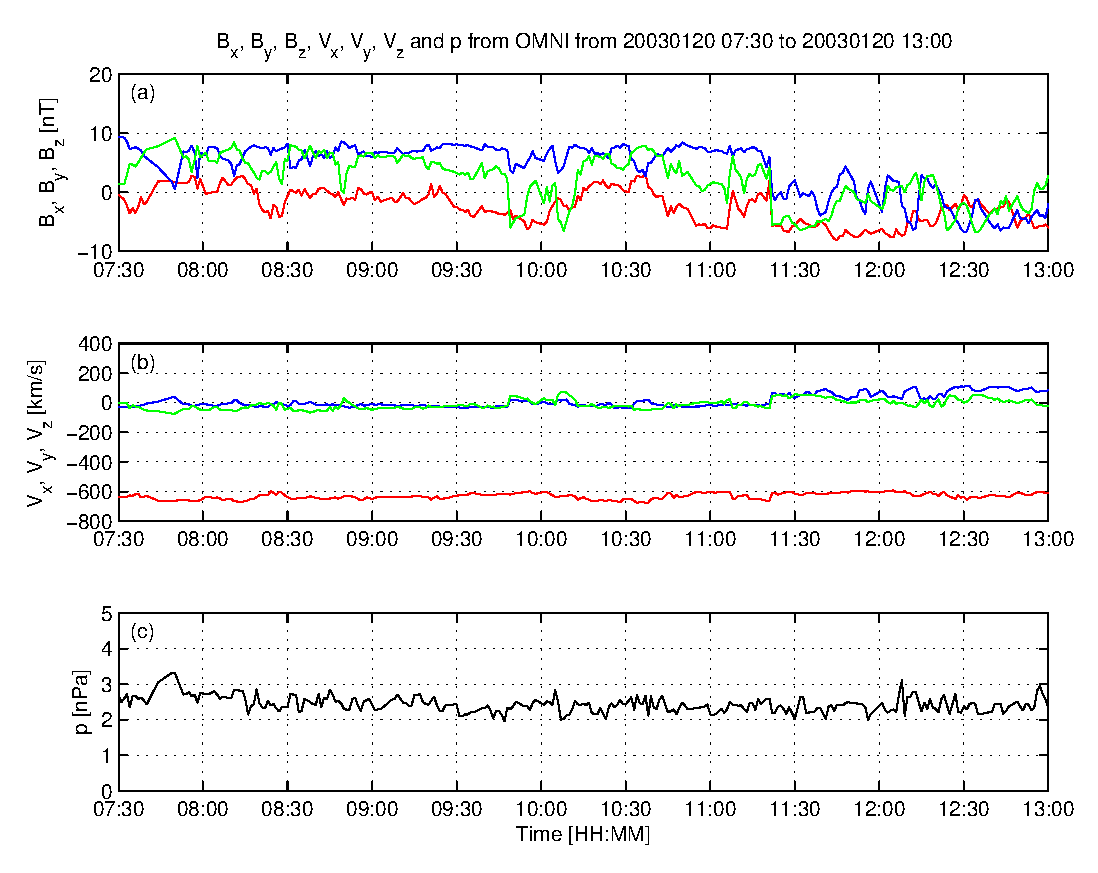
\includegraphics[width=0.9\textwidth,angle=0]{swe-2020-corr-f02.eps}  
\caption{OMNI solar wind data in GSE system from 7:30 to 13:00 (UT) on January 20, 2003. (a) Magnetic field $B_{x}$ (red), $B_{y}$ (green) and $B_{z}$ (blue) components. (b) Solar wind velocity $V_{x}$ (red), $V_{y}$ (green) and $V_{z}$ (blue) components. (c) The $P$ pressure of the solar wind (black).}

\label{fig:swomni}
\end{figure}

\pagebreak

\begin{figure}[h]
\centering
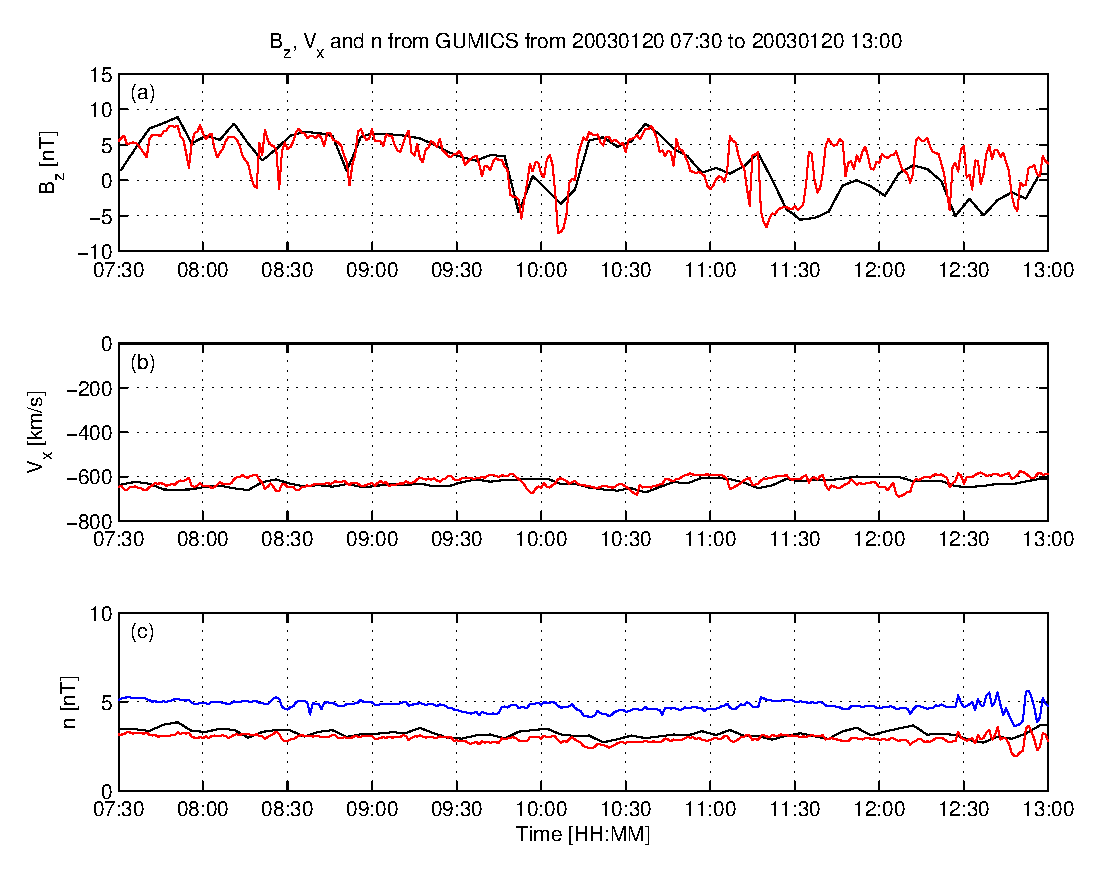
\includegraphics[width=0.9\textwidth,angle=0]{swe-2020-corr-f03.eps}  
\caption{GUMICS-4 simulation results (black) and Cluster SC3 magnetic field, ion plasma moments (red) and electron density calculated from spacecraft potential (blue) from January 20, 2003 from 7:30 to 13:00 (UT) in the solar wind in GSE system. (a) Magnetic field Z component. (b) Solar wind velocity X component (c) Solar wind density.}
\label{fig:swplot}
\end{figure}

\pagebreak

\begin{figure}[h]
\centering
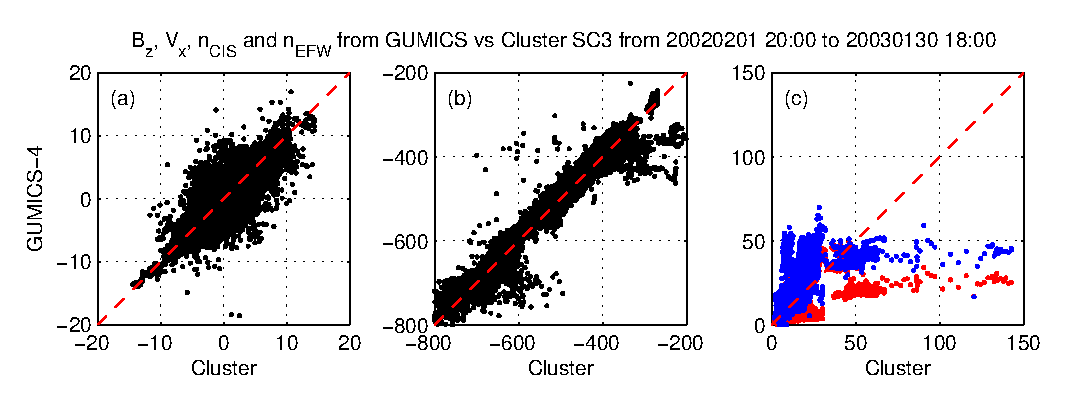
\includegraphics[width=0.9\textwidth,angle=0]{swe-2020-corr-f04.eps}
\caption{Scattered plots of the Cluster SC3 and GUMICS$-$4 simulations for all intervals in the solar wind. The dashed line is the y=x line. (a) Magnetic field Z component in GSE system. (b) Solar wind velocity X component in GSE system. (c) Solar wind density measured by the CIS HIA instrument (red) and calculated from the spacecraft potential (blue).}
\label{fig:swscatplot}
\end{figure}

\pagebreak

\begin{figure}[h]
\centering
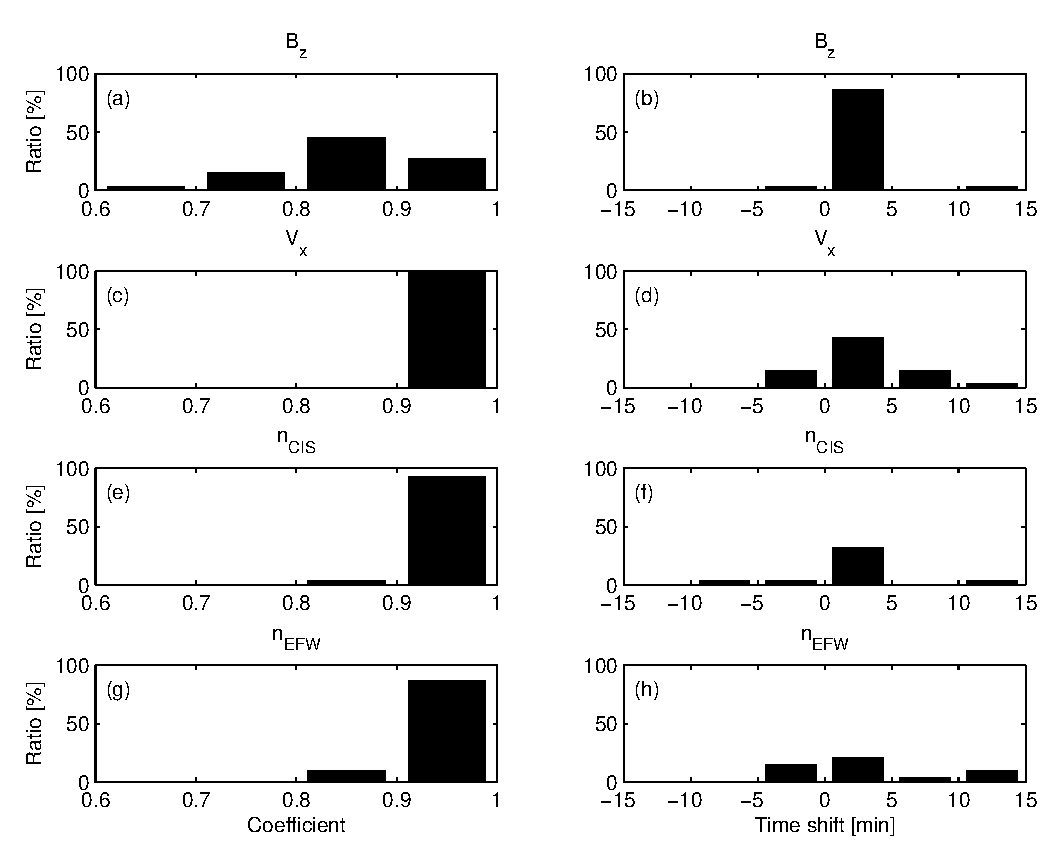
\includegraphics[width=0.9\textwidth,angle=0]{swe-2020-corr-f05.eps}  
\caption{The distributions of the correlation coefficients (a,~c,~e,~g) of the magnetic field Z component ($B_z$) in GSE system, solar wind velocity X component ($V_X$) in GSE system, the solar wind density measured by the CIS HIA ($n_{CIS}$) instrument and calculated from the spacecraft potential ($n_{EFW}$), respectively, for all intervals in the solar wind. The distributions of the time shifts (b,~d,~f,~h) of the $B_z$, the $V_X$, the $n_{CIS}$ and the $n_{EFW}$), respectively, for all intervals in the solar wind.}
\label{fig:swcorrplot}
\end{figure}

\pagebreak

\begin{figure}[h]
\centering
\includegraphics[width=0.9\textwidth,angle=0]{swe-2020-corr-f06.eps}  
\caption{Cluster SC3 orbit in the magnetosheath in GSE system for all intervals (see Table~\ref{tab:msh}). (a) XZ (b) YZ (c) XY (d) Cylindrical projection. Average bow-shock and magnetopause positions are drawn on all plots using solid line \citep[][respectively]{peredo95:_three_alfven_mach,tsyganenko95:_model_earth}. The black dots at $3.7\,R_E$ show the boundary of the GUMICS$-$4 inner magnetospheric domain. The black circle in the origo of all plots shows the size of the Earth.}
\label{fig:mshorbit}
\end{figure}

\pagebreak

\begin{figure}[h]
\centering
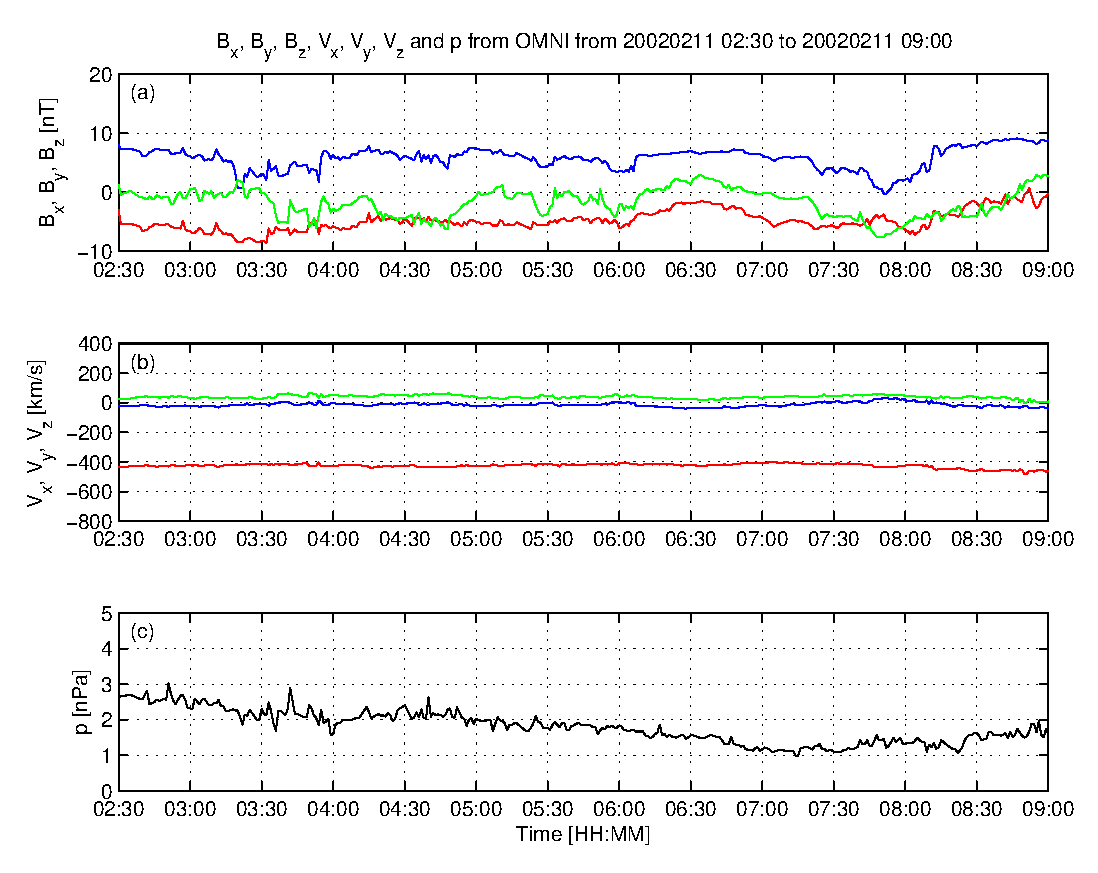
\includegraphics[width=0.9\textwidth,angle=0]{swe-2020-corr-f07.eps}  
\caption{OMNI solar wind data in GSE system from 2:30 to 09:00 (UT) on February 11, 2002. (a) Magnetic field $B_{x}$ (red), $B_{y}$ (green) and $B_{z}$ (blue) components. (b) Solar wind velocity $V_{x}$ (red), $V_{y}$ (green) and $V_{z}$ (blue) components. (c) The $P$ pressure of the solar wind (black).}
\label{fig:mshomni}
\end{figure}

\pagebreak

\begin{figure}[h]
\centering
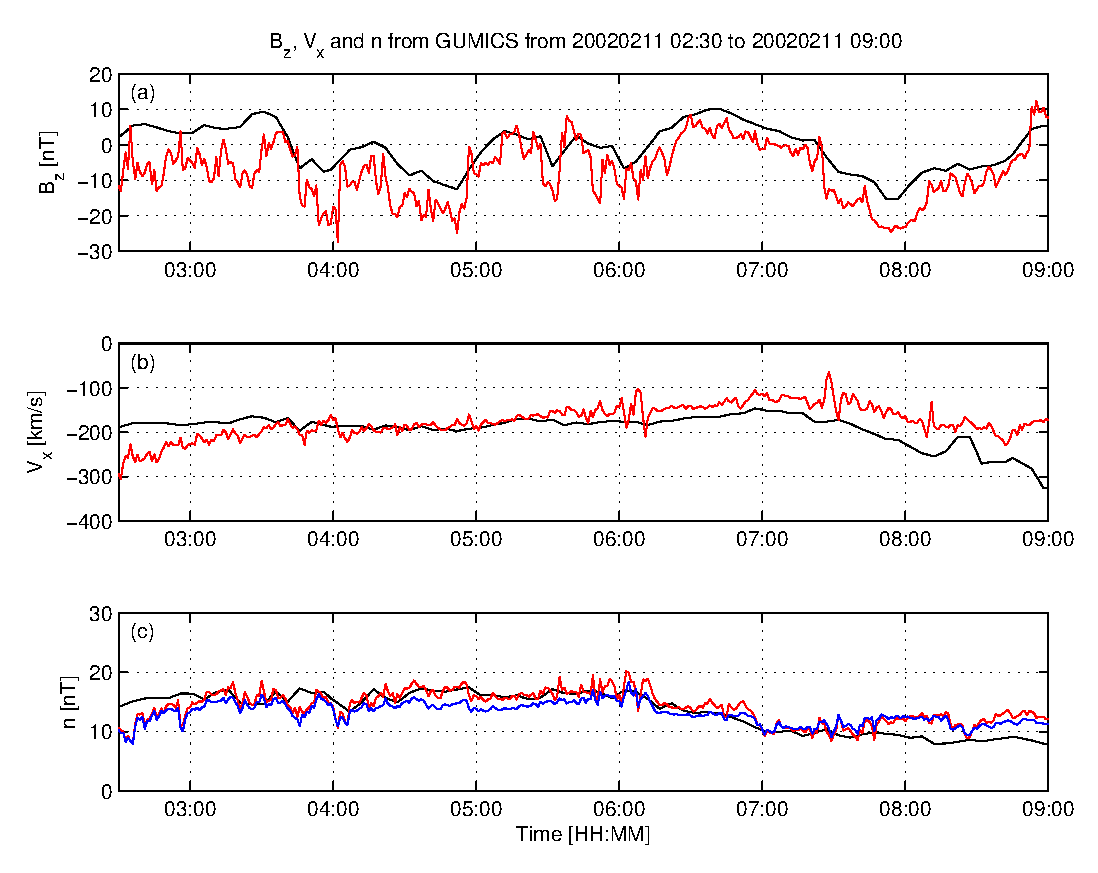
\includegraphics[width=0.9\textwidth,angle=0]{swe-2020-corr-f08.eps}  
\caption{GUMICS-4 simulation results (black) and Cluster SC3 magnetic field, ion plasma moments (red) and electron density calculated from spacecraft potential (blue) from February 11, 2002 from 2:30 to 9:00 (UT) in the magnetosheath in GSE system  (a) Magnetic field Z component. (b) Solar wind velocity X component (c) Solar wind density.}
\label{fig:mshplot}
\end{figure}

\pagebreak

\begin{figure}[h]
\centering
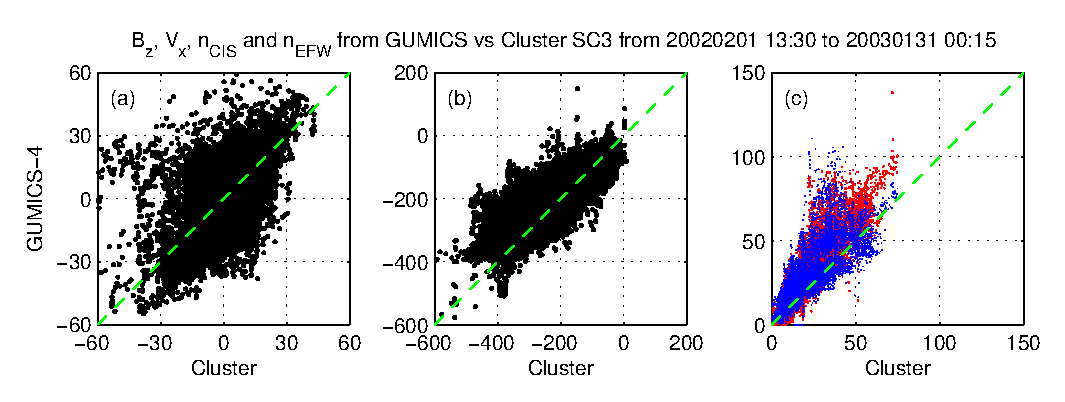
\includegraphics[width=0.9\textwidth,angle=0]{swe-2020-corr-f09.eps}
\caption{Scattered plots of the Cluster SC3 and GUMICS$-$4 simulations for all intervals in the magnetosheath in GSE system. The dashed line is the y=x line. (a) Magnetic field Z component. (b) Solar wind velocity X component. (c) Solar wind density measured by the CIS HIA instrument (red) and calculated from the spacecraft potential (blue).}
\label{fig:mshscatplot}
\end{figure}

\pagebreak

\begin{figure}[h]
\centering
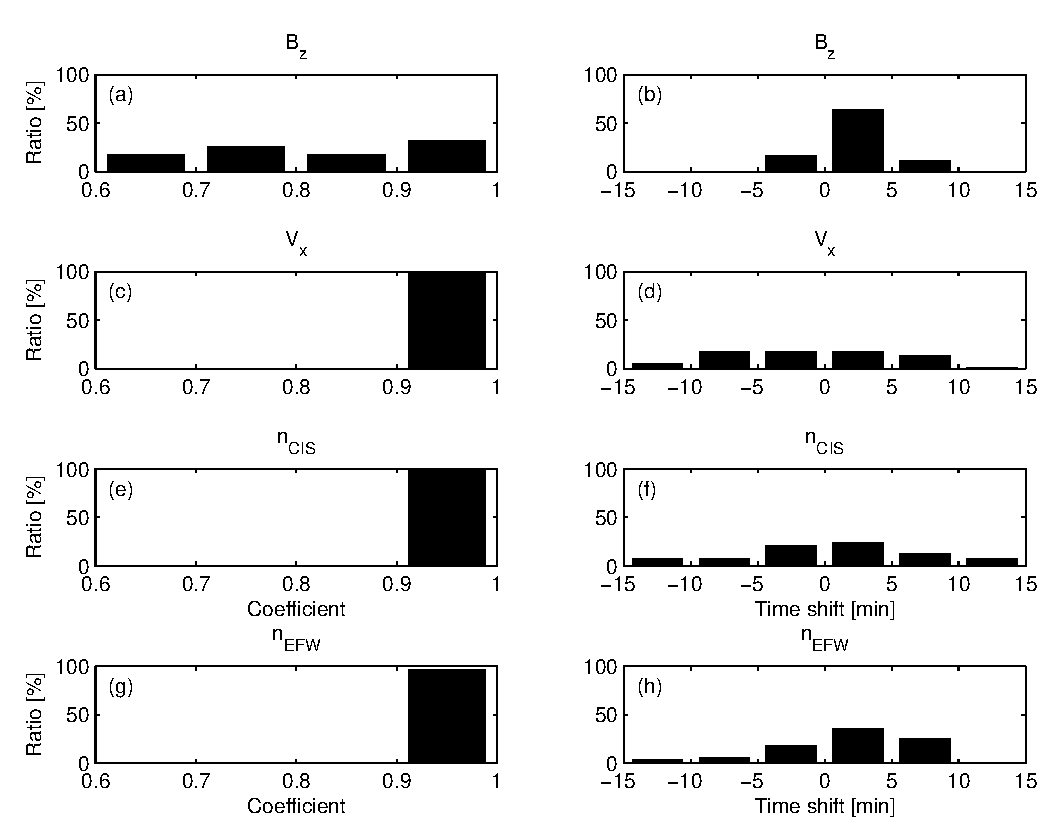
\includegraphics[width=0.9\textwidth,angle=0]{swe-2020-corr-f10.eps}
\caption{The distributions of the correlation coefficients (a,~c,~e,~g) of the magnetic field Z component ($B_z$) in GSE system, solar wind velocity X component ($V_X$) in GSE system, the solar wind density measured by the CIS HIA ($n_{CIS}$) instrument and calculated from the spacecraft potential ($n_{EFW}$), respectively, for all intervals in the magnetosheath. The distributions of the time shifts (b,~d,~f,~h) of the $B_z$, the $V_X$, the $n_{CIS}$ and the $n_{EFW}$), respectively, for all intervals in the magnetosheath.}
\label{fig:mshcorrplot}
\end{figure}

\pagebreak

\begin{figure}[h]
\centering
\includegraphics[width=0.9\textwidth,angle=0]{swe-2020-corr-f11.eps}  
\caption{Cluster SC3 orbit in the magnetosphere in GSE system for all intervals (see Table~\ref{tab:msph}). (a) XZ (b) YZ (c) XY (d) Cylindrical projection. Average bow-shock and magnetopause positions are drawn on all plots using solid line \citep[][respectively]{peredo95:_three_alfven_mach,tsyganenko95:_model_earth}. The black dots at $3.7\,R_E$ show the boundary of the GUMICS$-$4 inner magnetospheric domain. The black circle in the origo of all plots shows the size of the Earth.}
\label{fig:msphorbit}
\end{figure}

\pagebreak

\begin{figure}[h]
\centering
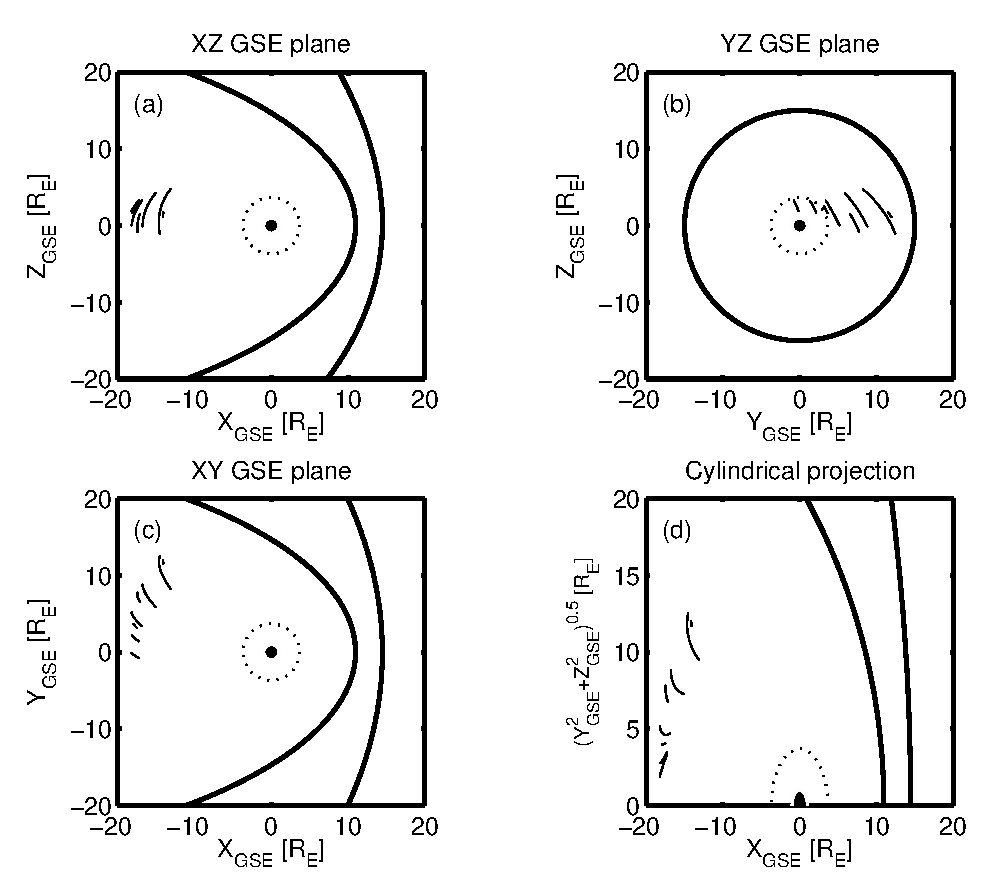
\includegraphics[width=0.9\textwidth,angle=0]{swe-2020-corr-f12.eps}  
\caption{Cluster SC3 orbit in the tail in GSE system for all intervals (see Table~\ref{tab:ns}). (a) XZ (b) YZ (c) XY (d) Cylindrical projection. Average bow-shock and magnetopause positions are drawn on all plots using solid line \citep[][respectively]{peredo95:_three_alfven_mach,tsyganenko95:_model_earth}. The black dots at $3.7\,R_E$ show the boundary of the GUMICS$-$4 inner magnetospheric domain. The black circle in the origo of all plots shows the size of the Earth.}
\label{fig:nsorbit}
\end{figure}

\pagebreak

\begin{figure}[h]
\centering
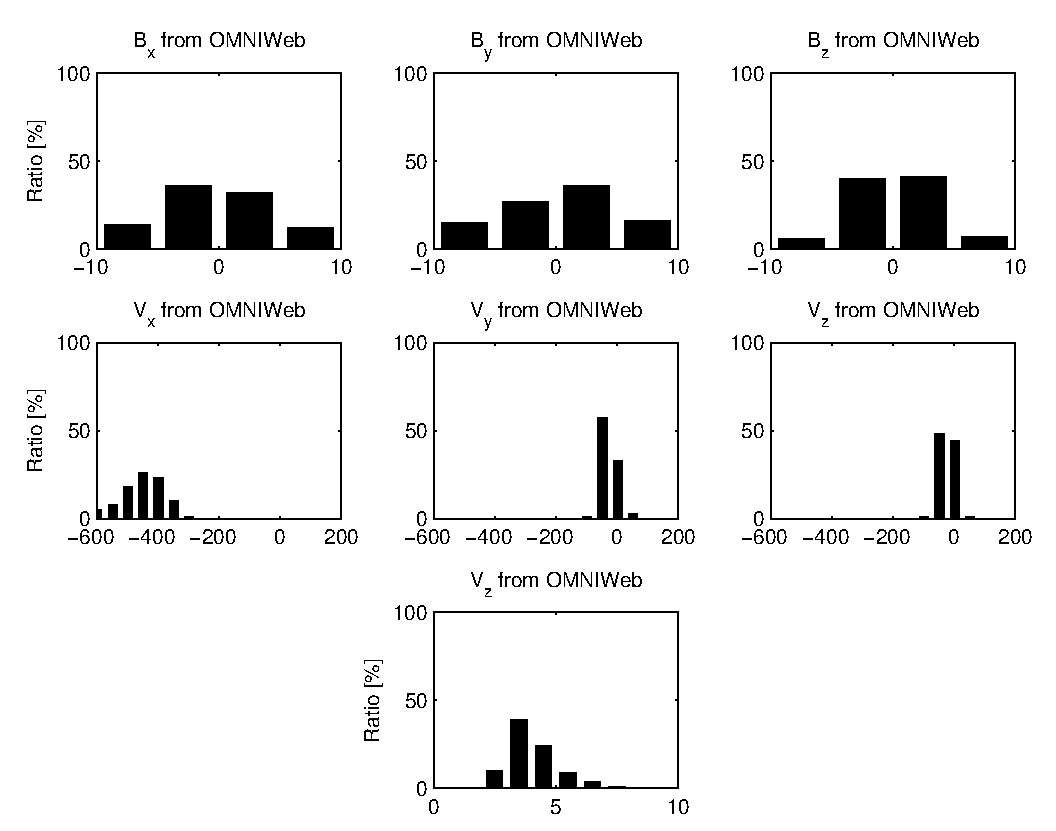
\includegraphics[width=0.9\textwidth,angle=0]{swe-2020-corr-f13.eps}  
\caption{(a, b, c) The distributions of the OMNI solar wind magnetic field ($B_{x}$, $B_{y}$, $B_{z}$) components, (d, e, f) the OMNI solar wind velocity ($V_{x}$, $V_{y}$, $V_{z}$) components and (g) the solar wind dynamic pressure during the 1-year run from January 29, 2002 to February 2, 2003 in GSE reference frame, respectively. The relative values are given on the vertical axis of all plots in percentage.}
\label{fig:omnidist}
\end{figure}

\pagebreak

\begin{figure}[h]
\centering
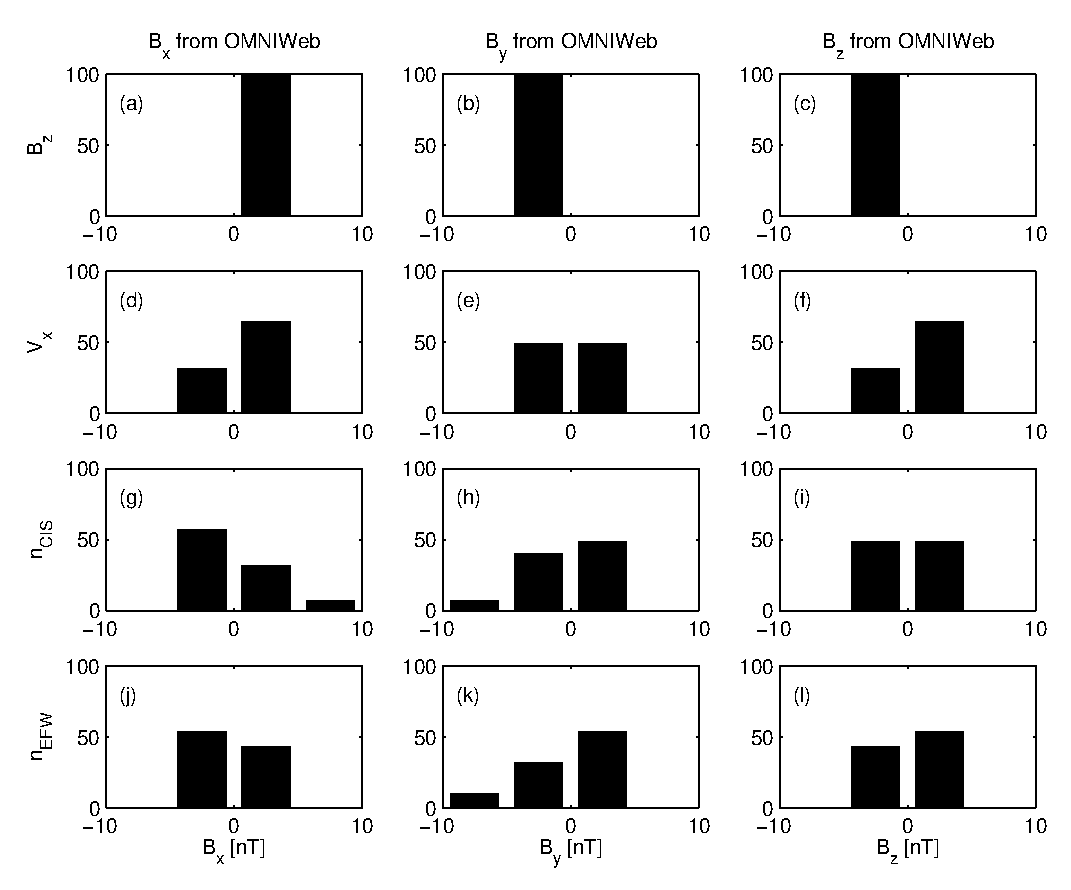
\includegraphics[width=0.9\textwidth,angle=0]{swe-2020-corr-f14.eps}  
\caption{The distributions of the $B_{x}$, the $B_{y}$  and the $B_{z}$ OMNI solar wind magnetic field components when the agreement of the Cluster SC3 measurements and the GUMICS$-$4 simulations are poor in the solar wind (see Table~\ref{tab:omnisw}). The $B_{z}$, the $V_{x}$, the $n_{CIS}$ and the $n_{EFW}$ are the magnetic field GSE Z component, the plasma ion velocity X GSE component, the  solar wind density measured by the CIS HIA instrument and the calculated from the EFW spacecraft potential, respectively. (a,~b,~c) Distribution of OMNI $B_{x}$, $B_{y}$, $B_{z}$ when the agreement of $B_{z}$ is poor. (d,~e,~f) Distribution of OMNI  $B_{x}$, $B_{y}$, $B_{z}$ when the agreement of $V_{x}$ is poor. (g,~h,~i) Distribution of OMNI $B_{x}$, $B_{y}$, $B_{z}$ when the agreement of $n_{CIS}$ is poor. (j,~k,~l) Distribution of OMNI $B_{x}$, $B_{y}$, $B_{z}$ when the agreement of $n_{EWF}$ is poor. The values are in percentage unit in the distributions.}
\label{fig:swomnibxyz}
\end{figure}

\pagebreak

\begin{figure}[h]
\centering
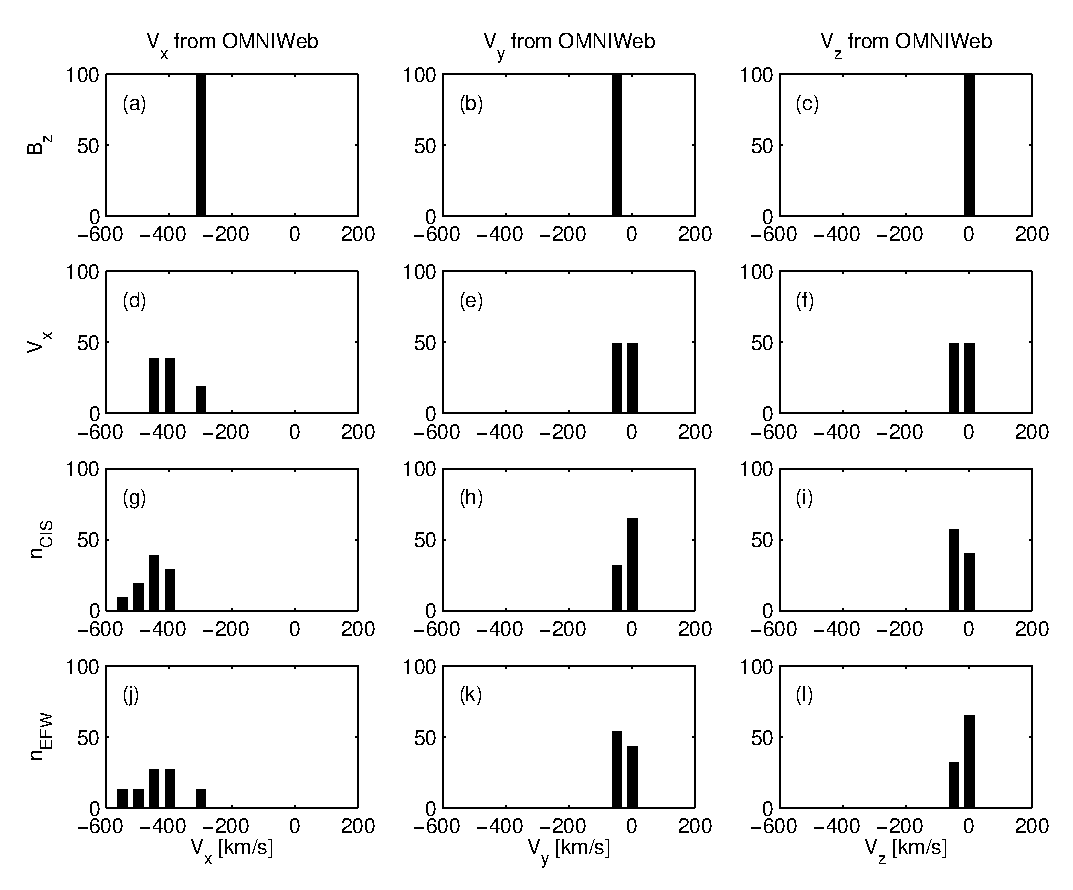
\includegraphics[width=0.9\textwidth,angle=0]{swe-2020-corr-f15.eps}
\caption{The distributions of the $V_{x}$, the $V_{y}$  and the $V_{z}$ OMNI solar wind magnetic field components when the agreement of the Cluster SC3 measurements and the GUMICS$-$4 simulations are poor in the solar wind (see Table~\ref{tab:omnisw}). The $B_{z}$, the $V_{x}$, the $n_{CIS}$ and the $n_{EFW}$ are the magnetic field GSE Z component, the plasma ion velocity X GSE component, the  solar wind density measured by the CIS HIA instrument and the calculated from the EFW spacecraft potential, respectively. (a,~b,~c) Distribution of OMNI $V_{x}$, $V_{y}$, $V_{z}$ when the agreement of $B_{z}$ is poor. (d,~e,~f) Distribution of OMNI  $V_{x}$, $V_{y}$, $V_{z}$ when the agreement of $V_{x}$ is poor. (g,~h,~i) Distribution of OMNI $V_{x}$, $V_{y}$, $V_{z}$ when the agreement of $n_{CIS}$ is poor. (j,~k,~l) Distribution of OMNI $V_{x}$, $V_{y}$, $V_{z}$ when the agreement of $n_{EWF}$ is poor. The values are in percentage unit in the distributions.}
\label{fig:swomnivxyz}
\end{figure}

\pagebreak

\begin{figure}[h]
\centering
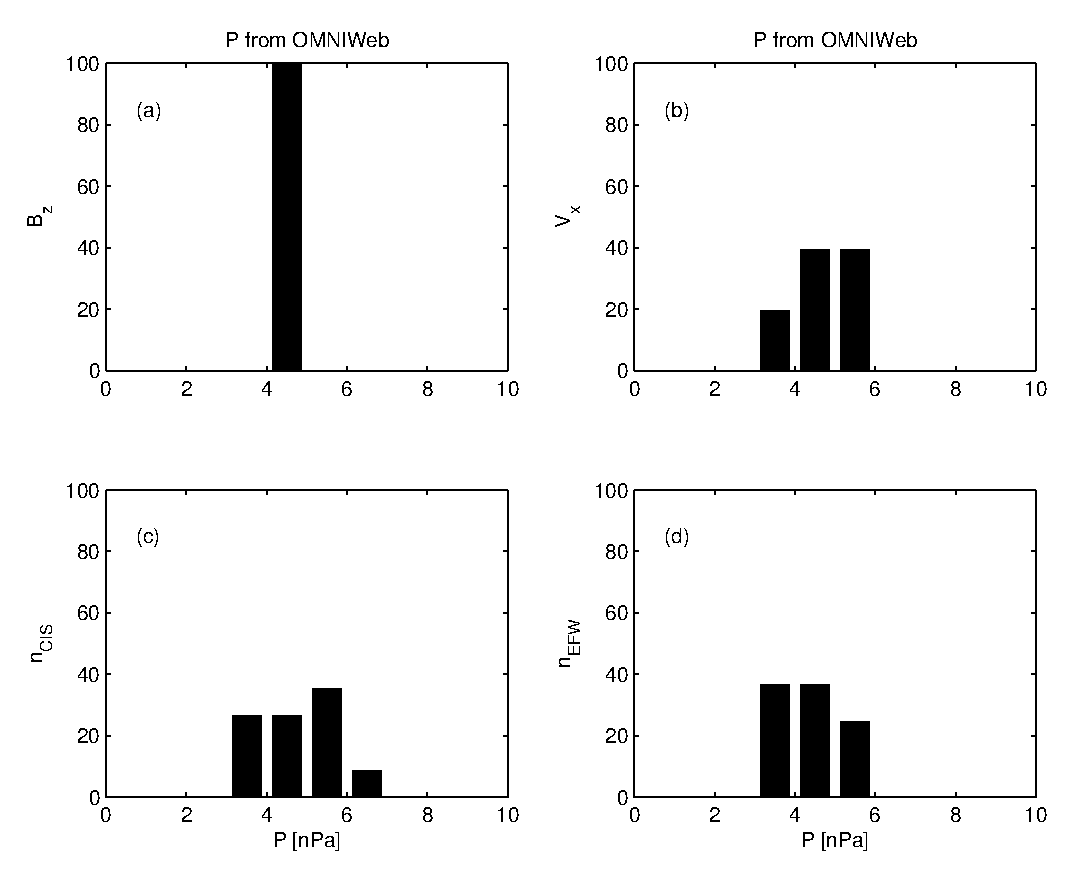
\includegraphics[width=0.9\textwidth,angle=0]{swe-2020-corr-f16.eps}  
\caption{The distributions of the $P$ solar wind dynamic pressure calculated from OMNI parameters when the agreement of the Cluster SC3 measurements and the GUMICS$-$4 simulations are poor in the solar wind (see Table~\ref{tab:omnisw}). The $B_{z}$, $V_{x}$, $n_{CIS}$ and $n_{EFW}$ are the magnetic field GSE Z component, the velocity X GSE component, the solar wind density measured by the CIS HIA instrument and calculated from the EFW spacecraft potential, respectively. (a,~b,~c,~d) The distribution of the P calculated from OMNI data when the agreement of the $B_{z}$, the $V_{x}$, the $n_{CIS}$ or the $n_{EFW}$ are poor. The values are in percentage unit in the distributions.}
\label{fig:swomnip}
\end{figure}

\pagebreak

\begin{figure}[h]
\centering
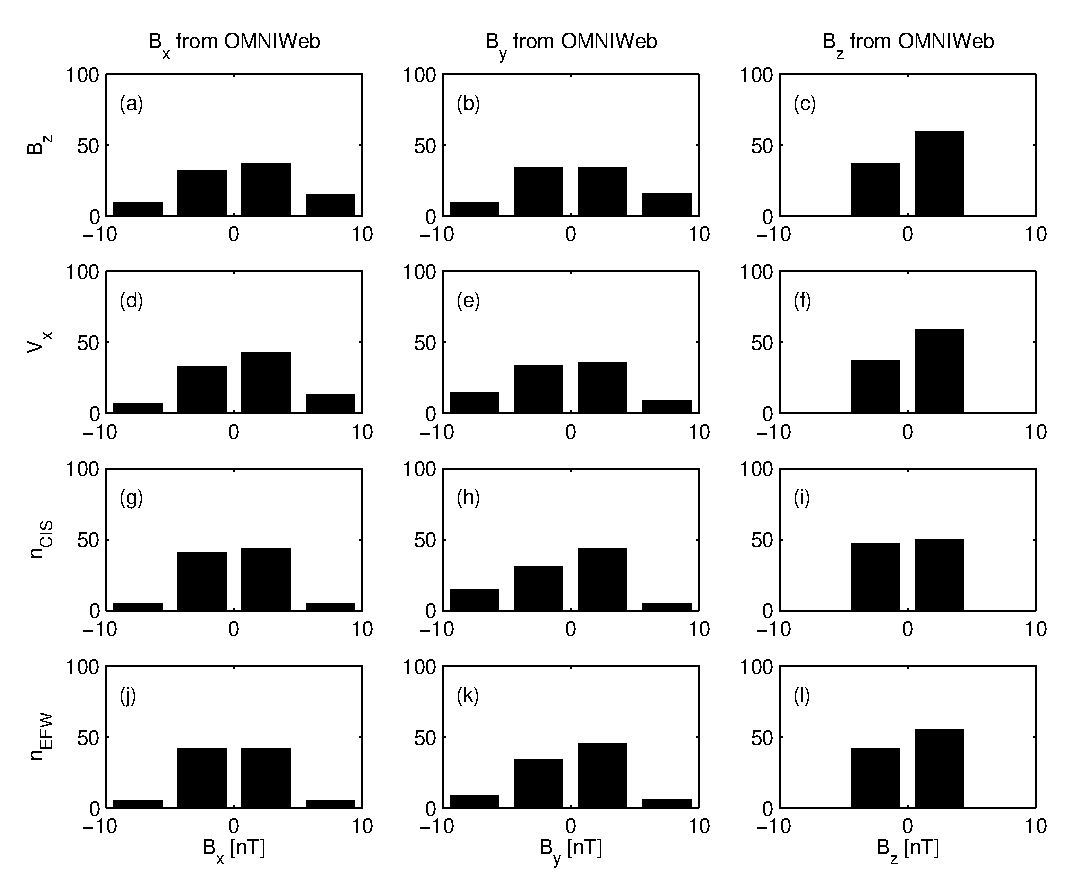
\includegraphics[width=0.9\textwidth,angle=0]{swe-2020-corr-f17.eps}
\caption{The distributions of the $B_{x}$, the $B_{y}$  and the $B_{z}$ OMNI solar wind magnetic field components when the agreement of the Cluster SC3 measurements and the GUMICS$-$4 simulations are poor in the magnetosheath (see Table~\ref{tab:omnimsh}). The $B_{z}$, the $V_{x}$, the $n_{CIS}$ and the $n_{EFW}$ are the magnetic field GSE Z component, the plasma ion velocity X GSE component, the  solar wind density measured by the CIS HIA instrument and the calculated from the EFW spacecraft potential, respectively. (a,~b,~c) Distribution of OMNI $B_{x}$, $B_{y}$, $B_{z}$ when the agreement of $B_{z}$ is poor. (d,~e,~f) Distribution of OMNI  $B_{x}$, $B_{y}$, $B_{z}$ when the agreement of $V_{x}$ is poor. (g,~h,~i) Distribution of OMNI $B_{x}$, $B_{y}$, $B_{z}$ when the agreement of $n_{CIS}$ is poor. (j,~k,~l) Distribution of OMNI $B_{x}$, $B_{y}$, $B_{z}$ when the agreement of $n_{EWF}$ is poor. The values are in percentage unit in the distributions.}
\label{fig:mshomnibxyz}
\end{figure}

\pagebreak

\begin{figure}[h]
\centering
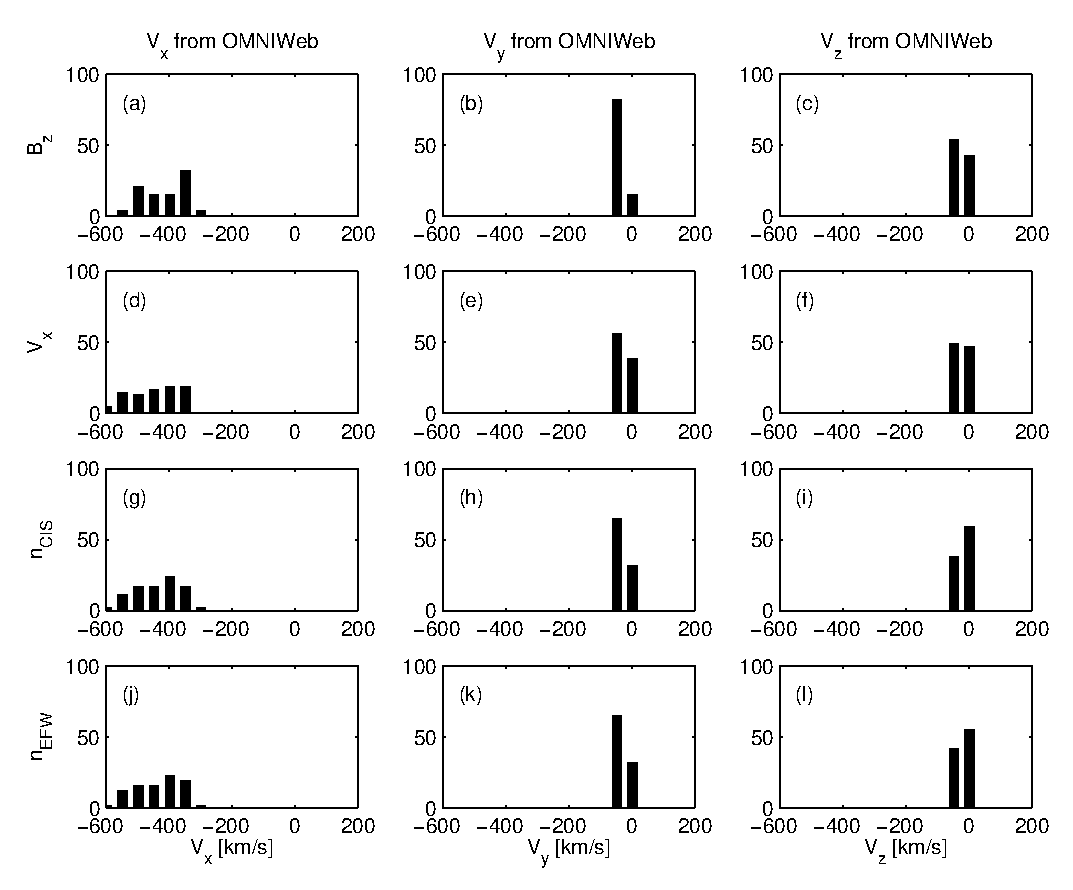
\includegraphics[width=0.9\textwidth,angle=0]{swe-2020-corr-f18.eps}
\caption{The distributions of the $V_{x}$, the $V_{y}$  and the $V_{z}$ OMNI solar wind magnetic field components when the agreement of the Cluster SC3 measurements and the GUMICS$-$4 simulations are poor in the magnetosheath (see Table~\ref{tab:omnimsh}). The $B_{z}$, the $V_{x}$, the $n_{CIS}$ and the $n_{EFW}$ are the magnetic field GSE Z component, the plasma ion velocity X GSE component, the  solar wind density measured by the CIS HIA instrument and the calculated from the EFW spacecraft potential, respectively. (a,~b,~c) Distribution of OMNI $V_{x}$, $V_{y}$, $V_{z}$ when the agreement of $B_{z}$ is poor. (d,~e,~f) Distribution of OMNI  $V_{x}$, $V_{y}$, $V_{z}$ when the agreement of $V_{x}$ is poor. (g,~h,~i) Distribution of OMNI $V_{x}$, $V_{y}$, $V_{z}$ when the agreement of $n_{CIS}$ is poor. (j,~k,~l) Distribution of OMNI $V_{x}$, $V_{y}$, $V_{z}$ when the agreement of $n_{EWF}$ is poor. The values are in percentage unit in the distributions.}
\label{fig:mshomnivxyz}
\end{figure}

\pagebreak

\begin{figure}[h]
\centering
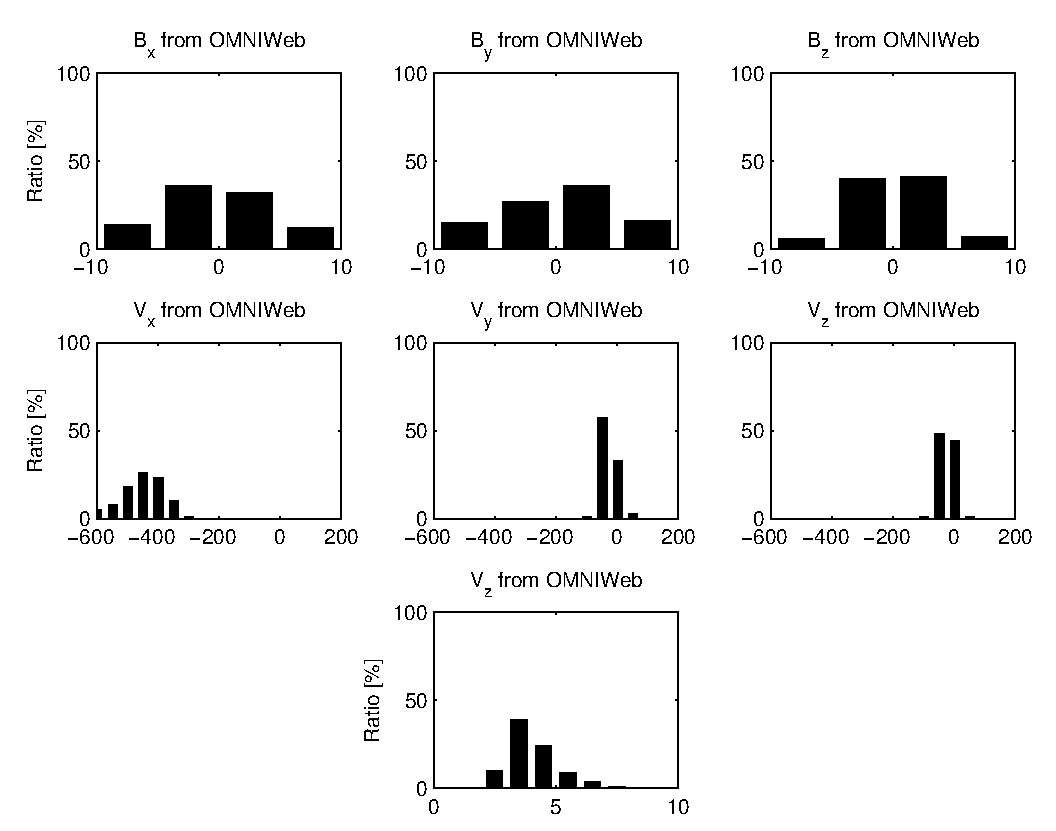
\includegraphics[width=0.9\textwidth,angle=0]{swe-2020-corr-f19.eps}
\caption{The distributions of the $P$ solar wind dynamic pressure calculated from OMNI parameters when the agreement of the Cluster SC3 measurements and the GUMICS$-$4 simulations are poor in the magnetosheath (see Table~\ref{tab:omnimsh}). The $B_{z}$, $V_{x}$, $n_{CIS}$ and $n_{EFW}$ are the magnetic field GSE Z component, the velocity X GSE component, the solar wind density measured by the CIS HIA instrument and calculated from the EFW spacecraft potential, respectively. (a,~b,~c,~d) The distribution of the P calculated from OMNI data when the agreement of the $B_{z}$, the $V_{x}$, the $n_{CIS}$ or the $n_{EFW}$ are poor. The values are in percentage unit in the distributions.}
\label{fig:mshomnip}
\end{figure}

\pagebreak

\begin{figure}[h]
\centering
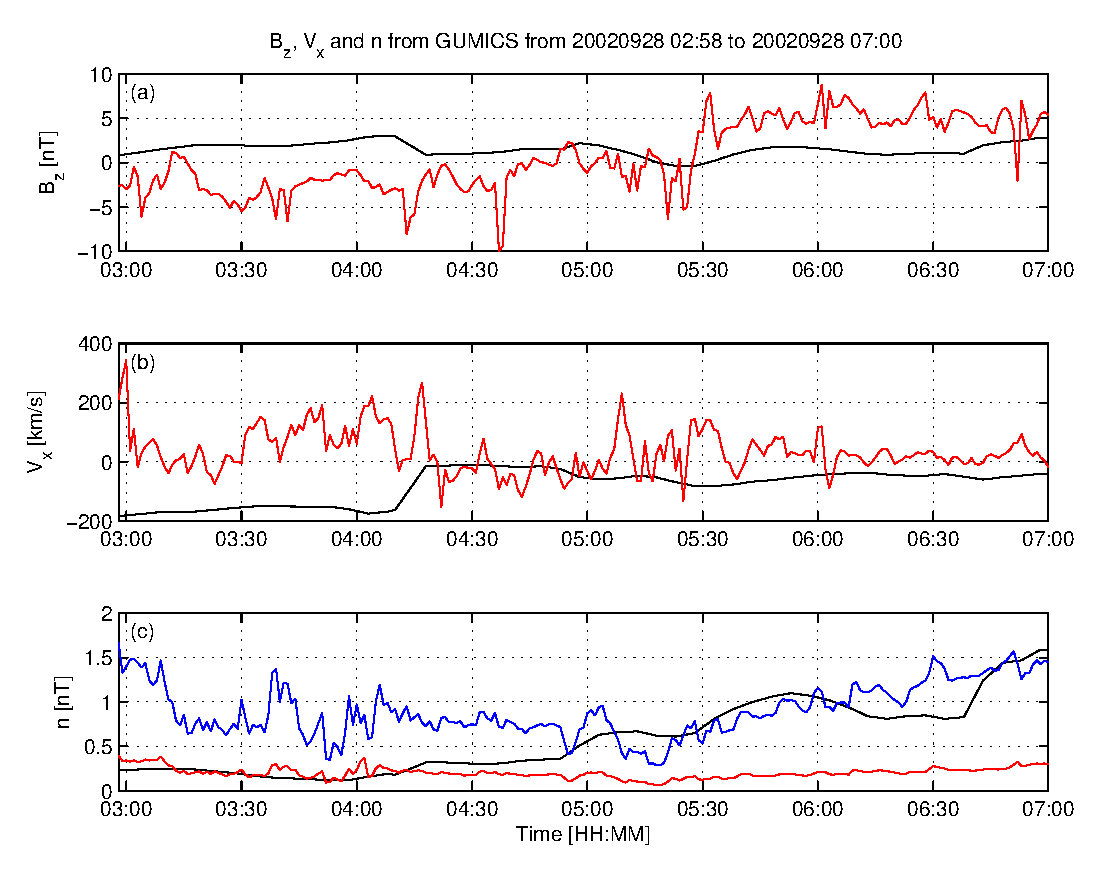
\includegraphics[width=0.9\textwidth,angle=0]{swe-2020-corr-f20.eps}  
\caption{GUMICS-4 simulation results (black) and Cluster SC3 magnetic field, ion plasma moments (red) and electron density calculated from spacecraft potential (blue) from September 28, 2002 from 2:58 to 7:00 (UT) in the tail in GSE system. (a) Magnetic field Z component. (b) Solar wind velocity X component (c) Solar wind density.}
\label{fig:nsplot}
\end{figure}

\pagebreak

% --- Tables ---

\pagebreak

\begin{table}[h]
\setlength{\tabcolsep}{3pt}
\centering
\begin{tabular}{c||cc|cc|cc|cc}
\hline
Start/End & $C_{B_{z}}$ & $\delta t_{B_{z}}$ & $C_{V_{x}}$ & $\delta t_{V_{x}}$ & $C_{n_{CIS}}$ & $\delta t_{n_{CIS}}$ & $C_{n_{EFW}}$ & $\delta t_{n_{EFW}}$ \\
& & [min] & & [min] & & [min] & & [min] \\
\hline
20020201 20:00/0203 04:00 & 0.96 & 2 & 1.00 & 13 & 0.96 & 3 & 0.98 & 3 \\
20020211 13:00/0212 12:00 & 0.82 & 2 & 1.00 & 0 & 0.99 & 18 & 0.99 & 18 \\
20020218 09:00/0219 02:00 & 0.93 & 0 & 1.00 & -3 & 0.94 & -3 & 0.97 & -3 \\
20020219 06:30/0219 15:00 & 0.93 & 1 & 1.00 & 0 & 0.99 & -60 & 1.00 & -52 \\
20020220 18:30/0222 00:00 & 0.87 & 4 & 1.00 & 4 & 0.93 & -21 & 0.98 & 3 \\
20020318 17:30/0319 02:30 & 0.89 & 1 & 1.00 & 21 & 0.98 & 50 & 0.99 & 5 \\
20020412 20:30/0413 02:00 & 0.90 & 4 & 0.99 & -54 & 0.94 & 60 & 0.98 & 12 \\
20021227 12:00/1228 03:00 & 0.75 & 4 & 1.00 & -3 & 0.99 & -26 & 0.99 & 21 \\
20021229 20:00/1230 16:00 & 0.68 & 1 & 1.00 & 1 & 0.99 & -30 & 0.98 & 41 \\
20030106 06:00/0106 19:00 & 0.79 & 4 & 1.00 & 6 & 0.99 & 4 & 0.99 & -60 \\
20030108 07:00/0109 03:30 & 0.55 & 10 & 1.00 & 41 & 0.99 & 10 & 0.97 & -55 \\
20030113 08:30/0113 18:00 & 0.91 & 3 & 1.00 & 5 & 1.00 & 3 & 0.97 & -1 \\
20030120 07:30/0120 13:00 & 0.82 & 2 & 1.00 & 9 & 1.00 & -6 & 1.00 & -3 \\
20030122 12:00/0123 14:00 & 0.81 & 2 & 1.00 & 3 & 0.99 & 3 & 0.92 & -60 \\
20030124 18:00/0126 00:00 & 0.73 & 3 & 1.00 & 0 & 0.99 & -60 & 0.99 & 60 \\
20030127 16:00/0128 06:00 & 0.88 & -1 & 1.00 & -3 & 0.95 & 1 & 0.88 & 11 \\
20030129 12:00/0130 18:00 & 0.90 & 2 & 1.00 & 4 & 0.94 & -59 & 0.98 & 1 \\
\hline
\end{tabular}
\caption{The studied solar wind intervals.  The correlation coefficients ($C_{B_{z}}$, $C_{V_{x}}$, $C_{n_{CIS}}$, $C_{n_{EFW}}$) and time shift ($\delta t_{V_{x}}$, $\delta t_{n_{CIS}}$, $\delta t_{n_{EFW}}$) in minutes of the magnetic field GSE Z component ($B_z$), solar wind velocity X component ($V_x$), CIS and EFW densities ($n_{CIS}, n_{EFW}$).\label{tab:sw}}
\end{table}

\pagebreak

\begin{center}
\setlength{\tabcolsep}{3pt}
\begin{longtable}{c||cc|cc|cc|cc}
\caption{The studied magnetosheath intervals.  The correlation coefficients ($C_{B_{z}}$, $C_{V_{x}}$, $C_{n_{CIS}}$, $C_{n_{EFW}}$) and time shift ($\delta t_{V_{x}}$, $\delta t_{n_{CIS}}$, $\delta t_{n_{EFW}}$) in minutes of the magnetic field GSE Z component ($B_z$), solar wind velocity X component ($V_x$), CIS and EFW densities ($n_{CIS}, n_{EFW}$). In the empty slots the correlation calculation gives invalid result. \label{tab:msh}}\\
\hline
Start/End & $C_{B_{z}}$ & $\delta t_{B_{z}}$ & $C_{V_{x}}$ & $\delta t_{V_{x}}$ & $C_{n_{CIS}}$ & $\delta t_{n_{CIS}}$ & $C_{n_{EFW}}$ & $\delta t_{n_{EFW}}$ \\
& & [min] & & [min] & & [min] & & [min] \\
\hline
\endfirsthead
\multicolumn{9}{c}%
{\tablename\ \thetable\ -- \textit{Continued from previous page}} \\
\hline
Start/End & $C_{B_{z}}$ & $\delta t_{B_{z}}$ & $C_{V_{x}}$ & $\delta t_{V_{x}}$ & $C_{n_{CIS}}$ & $\delta t_{n_{CIS}}$ & $C_{n_{EFW}}$ & $\delta t_{n_{EFW}}$ \\
& & [min] & & [min] & & [min] & & [min] \\
\hline
\endhead
\hline \multicolumn{9}{r}{\textit{Continued on next page}} \\
\endfoot
\hline
\endlastfoot
20020201 13:30/0201 18:30 & 0.91 & 1 & 0.98 & 56 & 0.99 & 60 & 0.976 & 60 \\
20020208 18:15/0209 00:00 & 0.73 & 2 & 0.95 & 60 & 0.98 & -52 & 0.98 & -54 \\
20020211 02:30/0211 09:00 & 0.79 & 0 & 0.99 & -20 & 0.99 & -1 & 0.99 & 1 \\
20020212 16:30/0212 21:00 & 0.80 & 3 & 0.99 & 54 & 0.99 & 31 & 0.99 & 30 \\
20020219 17:30/0219 23:00 & 0.76 & 4 & 0.98 & 37 & 0.99 & 7 & 0.99 & 6 \\
20020222 23:00/0223 06:30 & 0.64 & 0 & 0.97 & -60 & 0.99 & -47 & 0.98 & -48 \\
20020227 16:30/0227 23:15 & 0.48 & 59 & 0.98 & -31 & 0.99 & -39 & 1.00 & -12 \\
20020310 18:30/0311 00:30 & 0.97 & 3 & 0.98 & 19 & 0.99 & 8 & 0.99 & -2 \\
20020311 14:00/0311 19:00 & 0.86 & 5 & 0.97 & 36 & 0.99 & -3 & 0.99 & -40 \\
20020406 19:00/0407 01:15 & 0.76 & 2 & 0.96 & -60 & 0.98 & -55 & 0.98 & -56 \\
20020410 17:30/0410 23:00 & 0.89 & 6 & 0.99 & -50 & 0.99 & 3 & 1.00 & 5 \\
20020411 11:30/0411 16:30 & 0.82 & 4 & 0.99 & 39 & 0.99 & 3 & 0.99 & 3 \\
20020418 18:30/0418 22:45 & 0.92 & 60 & 0.99 & -60 & 0.99 & 60 & 0.98 & 60 \\
20020421 04:30/0421 07:45 & 0.96 & 47 & 0.99 & -60 & 1.00 & -60 & 1.00 & -60 \\
20020422 11:45/0422 15:45 & 0.73 & -5 & 0.98 & -17 & 0.99 & -15 & 0.98 & -16 \\
20020423 08:30/0423 12:30 & 0.93 & 31 & 0.99 & 3 & 0.99 & 16 & 0.99 & 16 \\
20020430 12:30/0430 17:00 & 0.79 & 59 & 0.98 & 22 & 0.98 & -18 &  &  \\
20020505 07:00/0505 11:15 & 0.71 & 59 & 0.99 & -58 & 0.98 & -60 &  &  \\
20020506 19:15/0507 00:15 & 0.84 & -27 & 0.98 & -60 & 0.97 & -37 &  &  \\
20020507 17:30/0507 23:00 & 0.93 & 2 & 0.98 & -30 & 0.99 & -49 &  &  \\
20020514 22:45/0515 03:00 & 0.79 & 49 & 0.99 & 35 & 0.99 & 38 & 0.99 & 43 \\
20020517 07:00/0517 12:15 & 0.74 & -5 & 1.00 & -5 & 0.99 & -4 & 0.99 & -3 \\
20020518 13:30/0518 19:30 & 0.70 & 1 & 0.99 & 9 & 0.97 & -1 & 0.97 & -1 \\
20020519 20:00/0520 03:30 & 0.98 & 2 & 1.00 & -9 & 0.99 & -5 & 0.99 & -50 \\
20020520 10:45/0520 20:15 & 0.77 & 1 & 0.99 & -3 & 0.95 & -1 & 0.99 & -1 \\
20020522 02:00/0522 08:45 & 0.49 & 52 & 0.99 & 4 & 0.99 & 12 & 0.99 & 22 \\
20020527 02:15/0527 17:15 & 0.79 & -3 & 0.99 & -3 & 0.98 & 0 & 0.98 & 0 \\
20020530 05:00/0530 10:30 & 0.29 & 3 & 1.00 & -38 & 0.99 & 3 & 0.99 & 3 \\
20020601 19:30/0602 01:00 & 0.68 & -2 & 1.00 & 18 & 0.99 & -6 & 0.99 & -7 \\
20020602 21:45/0603 17:45 & 0.62 & -5 & 0.99 & -1 & 0.98 & 2 & 0.99 & 2 \\
20020605 10:30/0606 06:00 & 0.18 & 0 & 1.00 & -7 & 0.97 & 10 & 0.98 & 9 \\
20020607 18:00/0607 22:00 & 0.92 & -35 & 1.00 & -36 & 0.99 & 16 & 0.99 & 16 \\
20020608 01:15/0608 18:15 & 0.53 & -4 & 0.99 & -39 & 0.96 & -6 & 0.97 & -6 \\
20020610 01:30/0610 09:30 & 0.76 & 5 & 0.99 & 8 & 0.99 & -5 & 0.99 & -7 \\
20020610 11:00/0611 01:00 & 0.87 & -4 & 0.99 & -33 & 0.98 & 23 & 0.99 & 6 \\
20020612 18:30/0613 06:15 & 0.44 & -2 & 0.99 & -7 & 0.97 & 4 & 0.97 & -32 \\
20020615 07:00/0615 23:30 & & & 1.00 & 47 & 0.98 & -3 & 0.98 & -3 \\
20020617 05:00/0618 03:45 & 0.76 & 4 & 1.00 & 28 & 0.98 & 10 & 0.98 & 8 \\
20020620 04:00/0620 11:00 & 0.61 & -8 & 0.99 & -6 & 0.97 & 12 & 0.98 & 4 \\
20020622 14:30/0622 18:00 & 0.98 & 55 & 1.00 & 35 & 0.99 & 16 & 1.00 & 16 \\
20021201 04:15/1202 07:45 & 0.38 & 1 & 1.00 & 2 & 0.99 & 6 & 0.99 & 6 \\
20021203 15:30/1204 19:30 & 0.67 & 1 & 0.99 & 60 & 0.98 & 59 & 0.98 & 59 \\
20021207 00:30/1207 07:45 & 0.49 & 37 & 0.98 & -56 & 0.99 & -19 & 0.99 & -4 \\
20021208 09:30/1209 08:00 & 0.69 & 2 & 0.98 & -35 & 0.97 & 6 & 0.98 & 4 \\
20021212 23:30/1213 14:30 & 0.51 & 5 & 1.00 & 36 & 0.99 & -3 & 0.81 & -56 \\
20021213 21:15/1214 09:30 & 0.93 & 5 & 0.99 & -35 & 0.99 & -13 & 0.99 & -47 \\
20021215 12:45/1216 18:00 & 0.76 & 2 & 0.99 & -60 & 0.94 & -60 & 0.98 & 31 \\
20021217 16:30/1218 01:45 & 0.99 & 2 & 1.00 & -54 & 0.99 & 3 & 0.99 & 3 \\
20021220 01:30/1220 06:15 & 0.92 & 0 & 1.00 & 60 & 0.99 & 2 & 0.99 & 3 \\
20021223 02:15/1223 13:00 & 0.91 & 1 & 0.97 & 49 & 0.93 & 49 & 0.99 & -14 \\
20021223 14:00/1223 22:30 & 0.84 & 1 & 0.99 & -2 & 0.99 & -1 & 1.00 & -3 \\
20021224 19:00/1225 01:45 & 0.94 & 0 & 1.00 & -44 & 0.99 & 26 & 0.99 & 27 \\
20021225 23:45/1226 07:15 & 0.96 & 7 & 1.00 & -17 & 0.99 & 56 & 0.99 & 55 \\
20021226 23:00/1227 09:45 & 0.79 & 2 & 1.00 & 2 & 0.98 & 4 & 0.99 & 3 \\
20021229 11:45/1229 17:00 & 0.60 & 2 & 1.00 & -60 & 0.98 & -19 & 0.98 & 50 \\
20021230 17:45/1231 01:00 & 0.69 & 1 & 0.98 & 52 & 0.98 & 60 & 0.98 & 22 \\
20021231 23:00/0101 05:15 & 0.89 & 2 & 0.99 & 15 & 0.99 & -54 & 1.00 & -58 \\
20030105 14:00/0105 21:00 & 0.69 & 0 & 0.99 & 1 & 0.98 & -60 & 0.99 & -60 \\
20030106 23:15/0107 03:00 & 0.52 & 9 & 0.98 & 60 & 0.99 & 56 & 1.00 & -60 \\
20030109 08:45/0109 16:15 &  &  & 0.91 & -56 & 0.98 & -13 & 0.98 & -26 \\
20030110 07:15/0110 15:15 & 0.94 & 1 & 0.99 & -7 & 0.99 & 1 & 0.98 & 5 \\
20030111 08:15/0111 22:30 & 0.84 & 0 & 0.99 & -59 & 0.94 & -15 & 0.94 & 8 \\
20030112 17:30/0113 00:15 & 0.98 & 0 & 1.00 & -52 & 0.99 & 39 & 0.99 & 51 \\
20030114 00:30/0114 08:30 & 0.84 & -1 & 0.99 & -60 & 0.98 & 23 & 0.98 & 8 \\
20030116 10:15/0116 17:45 & 0.62 & 60 & 0.93 & 52 & 0.99 & 60 & 0.99 & 30 \\
20030117 09:30/0117 13:30 & 0.68 & -3 & 1.00 & 8 & 1.00 & -31 & 0.99 & -33 \\
20030118 23:30/0119 03:45 & 0.93 & 3 & 1.00 & -12 & 1.00 & 7 & 0.99 & 7 \\
20030119 21:00/0120 01:00 & 0.94 & 3 & 1.00 & 5 & 1.00 & 38 & 1.00 & 19 \\
20030121 06:30/0121 11:30 & 0.82 & -15 & 0.96 & 47 & 0.98 & 7 & 0.99 & -39 \\
20030122 04:45/0122 09:30 & 0.69 & -2 & 1.00 & 10 & 0.99 & -9 & 0.99 & -5 \\
20030126 01:45/0126 06:30 & 0.85 & 3 & 0.99 & -15 & 0.99 & -50 & 0.99 & 23 \\
20030127 08:15/0127 13:00 & 1.00 & 9 & 1.00 & -60 & 0.98 & 0 & 0.99 & 1 \\
20030128 12:30/0128 17:15 & 0.77 & 60 & 0.99 & -24 & 0.99 & -6 & 0.988 & 20 \\
20030130 19:45/0131 00:15 & 0.98 & 2 & 0.99 & 51 & 0.99 & 25 & 0.99 & 9 \\
\end{longtable}
\end{center}

\pagebreak

\begin{center}
\setlength{\tabcolsep}{3pt}
\begin{longtable}{c}
\caption{The studied magnetosphere intervals (UT).\label{tab:msph}}\\
\hline
Start/End\\
\hline
\endfirsthead
\multicolumn{1}{c}%
{\tablename\ \thetable\ -- \textit{Continued from previous page}} \\
\hline
Start/End\\
\hline
\endhead
\hline \multicolumn{1}{r}{\textit{Continued on next page}} \\
\endfoot
\hline
\endlastfoot
20020213 23:00/0214 01:30 \\
20020217 18:30/0218 02:00 \\
20020220 00:45/0220 12:00 \\
20020222 11:15/0222 20:15 \\
20020225 02:15/0225 08:30 \\
20020227 06:00/0227 12:00 \\
20020302 00:00/0302 03:15 \\
20020306 10:00/0306 18:30 \\
20020308 17:30/0309 06:00 \\
20020311 02:15/0311 12:00 \\
20020313 11:15/0314 00:15 \\ 
20020316 04:45/0316 08:00 \\
20020318 09:00/0318 14:45 \\ 
20020320 20:30/0320 23:55 \\
20020323 04:00/0323 09:45 \\
20020327 23:45/0328 06:15 \\
20020330 07:15/0330 12:45 \\ 
20020401 19:30/0401 22:00 \\
20020406 09:30/0406 18:00 \\
20020408 15:00/0409 00:00 \\
20020410 23:30/0411 09:45 \\
20020413 08:30/0413 19:00 \\ 
20020416 18:00/0417 04:30 \\
20020418 06:00/0418 12:00 \\
20020420 15:00/0420 23:00 \\
20020422 20:00/0423 07:00 \\
20020425 08:30/0425 18:00 \\
20020430 04:40/0430 12:00 \\
20020504 14:30/0504 16:45 \\
20020505 02:30/0505 07:00 \\
20020507 01:30/0507 15:45 \\
20020508 11:00/0510 04:15 \\
20020512 02:45/0512 09:30 \\
20020514 10:30/0514 12:45 \\
20020519 00:30/0519 19:30 \\
20020521 01:30/0521 22:00 \\
20020523 23:30/0524 02:00 \\
20020524 19:00/0525 08:15 \\
20020526 07:30/0526 10:30 \\
20020528 20:00/0529 05:00 \\
20020531 02:15/0531 13:30 \\
20020602 04:30/0602 07:30 \\
20020602 12:00/0602 21:30 \\
20020604 08:30/0605 07:00 \\
20020606 14:30/0607 16:30 \\
20020609 06:00/0609 20:00 \\
20020611 11:00/0612 13:00 \\
20020614 01:00/0614 16:00 \\
20020616 08:00/0616 18:00 \\
20020620 13:30/0622 01:00 \\
20020623 13:00/0623 17:00 \\
20020624 04:00/0624 10:15 \\
20020630 17:45/0701 15:00 \\
20020701 21:00/0703 10:30 \\
20020703 23:00/0706 03:15 \\
20020707 01:00/0708 23:00 \\
20020710 11:30/0714 03:30 \\
20020714 15:45/0715 15:30 \\
20020716 23:30/0717 16:00 \\
20020718 05:45/0722 11:00 \\
20020722 23:45/0728 01:00 \\ 
20020728 02:00/0804 03:45 \\ 
20020804 04:45/0811 06:15 \\ 
20020811 07:30/0816 01:00 \\ 
20020816 15:30/0818 09:00 \\
20020818 10:00/0825 11:30 \\ 
20020825 13:00/0901 14:15 \\ 
20020901 17:15/0903 23:30 \\ 
20020905 02:15/0906 16:30 \\ 
20020907 10:30/0908 17:00 \\ 
20020908 18:00/0915 19:30 \\ 
20020915 21:00/0922 22:30 \\ 
20020923 00:00/0923 23:30 \\
20020924 03:30/0928 22:45 \\ 
20020928 23:30/0930 01:00 \\
20020930 02:15/1006 17:00 \\ 
20021006 17:45/1007 03:30 \\
20021007 05:00/1007 17:30 \\
20021008 07:30/1010 22:00 \\ 
20021010 22:30/1012 22:30 \\
20021012 23:00/1014 06:30 \\
20021014 09:00/1016 04:00 \\ 
20021016 14:00/1019 00:15 \\ 
20021019 01:30/1019 22:00 \\
20021021 04:00/1022 19:30 \\
20021022 22:30/1026 02:30 \\
20021026 04:00/1029 20:15 \\
20021030 01:30/1102 08:00 \\
20021102 22:00/1104 22:00 \\
20021106 00:00/1107 18:00 \\
20021108 02:00/1109 18:45 \\
20021111 00:00/1112 01:30 \\
20021113 03:45/1114 14:15 \\
20021115 20:30/1116 23:00 \\
20021118 01:00/1118 23:30 \\
20021120 17:00/1121 06:00 \\
20021122 21:30/1124 01:00 \\
20021125 04:00/1126 08:30 \\
20021127 20:00/1128 18:30 \\
20021130 04:00/1201 01:30 \\
20021202 14:30/1203 09:00 \\
20021204 22:00/1205 19:30 \\
20021207 09:00/1207 16:30 \\
20021207 18:00/1207 22:00 \\
20021209 16:30/1210 14:30 \\
20021212 13:45/1212 21:30 \\
20021214 13:30/1214 20:00 \\
20021214 21:00/1215 07:30 \\
20021216 21:00/1217 15:00 \\
20021219 08:00/1219 19:30 \\
20021221 15:45/1221 23:15 \\
20021222 00:30/1222 08:45 \\
20021224 02:30/1224 14:00 \\
20021226 10:00/1226 19:00 \\
20021228 19:30/1229 02:30 \\
20021229 04:00/1229 10:00 \\
20021231 05:00/1231 18:45 \\
20030102 12:30/0102 20:45 \\
20030104 20:45/0105 06:00 \\
20030105 07:00/0105 13:30 \\
20030107 05:45/0107 21:00 \\
20030109 17:00/0110 00:45 \\
20030112 00:00/0112 09:15 \\
20030112 10:30/0112 16:00 \\
20030114 11:00/0114 20:00 \\
20030116 20:30/0116 22:45 \\
20030119 04:30/0119 09:30 \\
20030119 14:00/0119 17:00 \\
20030121 13:30/0121 21:30 \\
20030126 07:30/0126 15:45 \\
20030128 17:45/0129 08:15 \\
20030131 01:30/0131 11:45 \\
\end{longtable}
\end{center}

\pagebreak

\begin{table}[!h]
%\setlength{\tabcolsep}{3pt}
\centering
\begin{tabular}{l|ccc|cccc}
\hline
& \multicolumn{3}{|c|}{OMNI} & \multicolumn{4}{|c}{Cluster SC3} \\  
Start/End & $B_{z}$ & $V_{x}$ & P & $B_{z}$ & $V_{x}$ & $n_{CIS}$ & $n_{EFW}$ \\
& [nT] & [km/s] & [$cm^{-3}$] \\
  \hline
20020201 20:00/0203 04:00 & -1.25 & -373.52 & 4.08 & y & y & n & y \\
20020211 13:00/0212 12:00 & 0.03 & -533.11 & 2.18 & y & y & y & y \\
20020218 09:00/0219 02:00 & 2.56 & -362.41 & 3.46 & y & n & n & y \\
20020219 06:30/0219 15:00 & 3.55 & -401.63 & 1.25 & y & y & n & n \\
20020220 18:30/0222 00:00 & 1.95 & -440.18 & 1.96 & y & y & n & y \\
20020318 17:30/0319 02:30 & 3.79 & -429.30 & 15.34 & y & n & n & n \\
20020412 20:30/0413 02:00 & -1.81 & -420.35 & 3.24 & y & n & n & y \\
20021227 12:00/1228 03:00 & 0.09 & -714.40 & 2.72 & y & n & n & y \\
20021229 20:00/1230 16:00 & -0.37 & -526.40 & 2.26 & y & y & n & n \\
20030106 06:00/0106 19:00 & 2.25 & -399.91 & 1.50 & y & n & n & n \\
20030108 07:00/0109 03:30 & -0.58 & -280.80 & 2.97 & n & n & y & n \\
20030113 08:30/0113 18:00 & 0.68 & -397.83 & 1.72 & y & y & y & n \\
20030120 07:30/0120 13:00 & 2.16 & -630.69 & 2.43 & y & y & y & y \\
20030122 12:00/0123 14:00 & 0.13 & -608.96 & 3.41 & y & y & y & n \\
20030124 18:00/0126 00:00 & -0.71 & -739.68 & 2.87 & y & y & n & n \\
20030127 16:00/0128 06:00 & -0.92 & -451.84 & 3.12 & y & y & n & n \\
20030129 12:00/0130 18:00 & -3.09 & -450.00 & 3.96 & y & y & n & y \\
\hline
\end{tabular}
\caption{The average OMNI input parameters in the solar wind and the good/bad agreement of the GUMICS$-$4 simulations to the Cluster $B_{z}$ magnetic field component, the $V_{x}$ solar wind speed component, the $n_{CIS}$ solar wind density measured by the Cluster CIS HIA instrument and the $n_{EFW}$ solar wind density calculated from the spacecraft potential measured by the Cluster EFW instrument in the solar wind.\label{tab:omnisw}}
\end{table}

\pagebreak

\begin{center}
\setlength{\tabcolsep}{3pt}
\begin{longtable}{l|rcc|cccc}
\caption{The average OMNI input parameters in the solar wind and the good/bad agreement of the GUMICS$-$4 simulations to the Cluster $B_{z}$ magnetic field component, the $V_{x}$ solar wind speed component, the $n_{CIS}$ solar wind density measured by the Cluster CIS HIA instrument and the $n_{EFW}$ solar wind density calculated from the spacecraft potential measured by the Cluster EFW instrument in the magnetosheath.\label{tab:omnimsh}}\\
\hline
& \multicolumn{3}{|c|}{OMNI} & \multicolumn{4}{|c}{Cluster SC3} \\  
Start/End & $B_{z}$ & $V_{x}$ & P & $B_{z}$ & $V_{x}$ & $n_{CIS}$ & $n_{EFW}$ \\
& [nT] & [km/s] & [$cm^{-3}$] \\
\hline
\endfirsthead
\multicolumn{1}{c}%
{\tablename\ \thetable\ -- \textit{Continued from previous page}} \\
\hline
& \multicolumn{3}{|c|}{OMNI} & \multicolumn{4}{|c}{Cluster SC3} \\  
Start/End & $B_{z}$ & $V_{x}$ & P & $B_{z}$ & $V_{x}$ & $n_{CIS}$ & $n_{EFW}$ \\
& [nT] & [km/s] & [$cm^{-3}$] \\
\hline
\endhead
\hline \multicolumn{1}{r}{\textit{Continued on next page}} \\
\endfoot
\hline
\endlastfoot
20020201 13:30/0201 18:30 & 0.19 & -342.87 & 4.62 & y & n & n & n \\
20020208 18:15/0209 00:00 & -0.48 & -508.16 & 1.61 & y & n & n & n \\
20020211 02:30/0211 09:00 & -1.85 & -425.67 & 1.78 & y & y & y & y \\
20020212 16:30/0212 21:00 &  2.98 & -509.22 & 2.34 & y & n & n & n \\
20020219 17:30/0219 23:00 & 1.46 & -431.50 & 1.46 & y & y & y & y \\
20020222 23:00/0223 06:30 & 0.86 & -391.22 & 1.14 & y & n & n & n \\
20020227 16:30/0227 23:15 & 1.89 & -343.13 & 1.52 & n & n & n & n \\
20020310 18:30/0311 00:30 & -2.81 & -379.46 & 1.78 & y & y & y & y \\
20020311 14:00/0311 19:00 & 1.63 & -371.43 & 2.68 & n & n & n & n \\
20020406 19:00/0407 01:15 & -2.71 & -333.13 & 0.93 & y & n & n & n \\
20020410 17:30/0410 23:00 & 0.31 & -312.43 & 4.42 & n & n & y & y \\
20020411 11:30/0411 16:30 & -1.50 & -494.02 & 4.25 & y & y & n & n \\
20020418 18:30/0418 22:45 & -0.92 & -450.82 & 0.30 & n & n & n & n \\
20020421 04:30/0421 07:45 & 0.40 & -455.69 & 1.37 & n & n & n & n \\
20020422 11:45/0422 15:45 & 0.25 & -419.98 & 1.14 & n & n & y & y \\
20020423 08:30/0423 12:30 & 2.77 & -507.99 & 6.82 & n & n & n & n \\
20020430 12:30/0430 17:00 & 2.15 & -479.51 & 3.02 & n & n & n & n \\
20020505 07:00/0505 11:15 & 0.20 & -336.81 & 1.74 & n & n & n & n \\
20020506 19:15/0507 00:15 & 0.78 & -390.00 & 2.46 & y & n & n & n \\
20020507 17:30/0507 23:00 & 2.87 & -392.40 & 3.49 & y & n & n & n \\
20020514 22:45/0515 03:00 & -2.42 & -414.01 & 1.82 & n & n & n & n \\
20020517 07:00/0517 12:15 & -0.39 & -379.32 & 1.52 & y & y & y & y \\
20020518 13:30/0518 19:30 & 0.63 & -345.87 & 1.59 & n & n & y & y \\
20020519 20:00/0520 03:30 & 4.75 & -408.56 & 1.12 & y & y & y & y \\
20020520 10:45/0520 20:15 & 0.74 & -448.89 & 1.93 & y & y & y & y \\
20020522 02:00/0522 08:45 & -1.07 & -398.12 & 1.63 & n & y & y & y \\
20020527 02:15/0527 17:15 & -3.11 & -542.53 & 2.07 & y & y & y & y \\
20020530 05:00/0530 10:30 & 0.03 & -493.86 & 2.08 & y & n & y & y \\
20020601 19:30/0602 01:00 & -3.38 & -342.27 & 4.16 & y & y & y & y \\
20020602 21:45/0603 17:45 & 0.38 & -435.47 & 1.89 & y & y & y & y \\
20020605 10:30/0606 06:00 & -0.42 & -394.49 & 1.08 & y & y & n & n \\
20020607 18:00/0607 22:00 & -1.60 & -291.85 & 1.80 & y & y & y & y \\
20020608 01:15/0608 18:15 & 0.06 & -335.39 & 2.74 & y & n & y & y \\
20020610 01:30/0610 09:30 & 1.60 & -465.52 & 3.00 & y & y & y & y \\
20020610 11:00/0611 01:00 & -2.27 & -419.86 & 2.16 & y & n & y & y \\
20020612 18:30/0613 06:15 & -1.13 & -351.03 & 1.16 & y & y & y & y \\
20020615 07:00/0615 23:30 & -1.16 & -334.27 & 2.84 & n & n & y & y \\
20020617 05:00/0618 03:45 & 0.78 & -351.47 & 1.87 & y & n & y & y \\
20020620 04:00/0620 11:00 & 0.46 & -485.48 & 1.73 & y & y & y & y \\
20020622 14:30/0622 18:00 & -0.72 & -429.02 & 1.93 & n & n & y & y \\
20021201 04:15/1202 07:45 & -1.09 & -499.23 & 2.62 & y & y & y & y \\
20021203 15:30/1204 19:30 & 0.34 & -449.09 & 2.06 & y & n & n & n \\
20021207 00:30/1207 07:45 & 0.80 & -451.80 & 7.33 & n & n & y & y \\
20021208 09:30/1209 08:00 & 0.60 & -600.27 & 1.49 & y & n & y & y \\
20021212 23:30/1213 14:30 & 0.10 & -337.77 & 1.32 & y & n & n & n \\
20021213 21:15/1214 09:30 & -0.74 & -361.19 & 2.99 & y & n & y & y \\
20021215 12:45/1216 18:00 & 1.32 & -479.48 & 1.53 & y & n & n & n \\
20021217 16:30/1218 01:45 & 4.56 & -393.99 & 2.49 & y & n & y & y \\
20021220 01:30/1220 06:15 & -1.21 & -530.62 & 3.01 & y & n & y & y \\
20021223 02:15/1223 13:00 & -2.32 & -516.12 & 2.22 & y & n & n & n \\
20021223 14:00/1223 22:30 & 0.89 & -519.77 & 2.55 & y & y & y & y \\
20021224 19:00/1225 01:45 & 0.88 & -523.86 & 3.41 & y & n & y & y \\
20021225 23:45/1226 07:15 & -0.61 & -414.38 & 2.21 & y & y & n & n \\
20021226 23:00/1227 09:45 & -1.79 & -618.14 & 6.20 & y & y & y & y \\
20021229 11:45/1229 17:00 & -0.41 & -580.12 & 2.39 & y & n & n & n \\
20021230 17:45/1231 01:00 & -1.01 & -483.60 & 1.93 & y & n & n & y \\
20021231 23:00/0101 05:15 & 0.60 & -418.95 & 1.94 & y & n & n & n \\
20030105 14:00/0105 21:00 & -0.03 & -414.46 & 1.69 & y & n & n & n \\
20030106 23:15/0107 03:00 & -1.62 & -392.29 & 1.56 & n & n & n & n \\
20030109 08:45/0109 16:15 & 1.45 & -272.82 &  2.31 & n & n & n & n \\
20030110 07:15/0110 15:15 & -2.11 & -401.03 & 2.72 & y & n & y & y \\
20030111 08:15/0111 22:30 & -0.20 & -433.33 & 1.24 & y & n & n & y \\
20030112 17:30/0113 00:15 & 1.53 & -389.62 & 1.45 & y & n & n & n \\
20030114 00:30/0114 08:30 & -1.67 & -388.53 & 2.27 & y & n & n & y \\
20030116 10:15/0116 17:45 & -1.20 & -328.91 & 1.22 & n & n & n & n \\
20030117 09:30/0117 13:30 & -1.36 & -327.09 & 2.55 & y & y & y & y \\
20030118 23:30/0119 03:45 & 6.41 & -459.46 & 4.82 & y & y & y & y \\
20030119 21:00/0120 01:00 & 1.52 & -597.95 & 2.38 & y & n & y & y \\
20030121 06:30/0121 11:30 & -1.77 & -670.25 & 1.50 & y & n & n & n \\
20030122 04:45/0122 09:30 & 0.11 & -588.87 & 2.30 & y & n & y & y \\
20030126 01:45/0126 06:30 & -0.24 & -713.82 & 2.75 & y & y & y & y \\
20030127 08:15/0127 13:00 & 7.94 & -509.30 & 0.47 & y & n & y & y \\
20030128 12:30/0128 17:15 & 4.95 & -443.83 & 4.15 & y & y & y & y \\
20030130 19:45/0131 00:15 & 4.21 & -510.33 & 2.63 & y & n & y & y \\
\hline
\end{longtable}
\end{center}

\pagebreak

\begin{table}[h]
\setlength{\tabcolsep}{3pt}
\centering
\begin{tabular}{lc}
\hline
Start/End & GUMICS Neutral Sheet\\
\hline
20020901 19:10/0901 23:54 & -- \\
20020906 14:07/0906 16:37 & + \\
20020913 17:33/0913 20:06 & + \\
20020918 12:47/0918 14:26 & -- \\
20020920 20:36/0921 02:13 & + \\
20020928 02:58/0928 07:00 & + \\
20021002 16:12/1002 23:52 & -- \\
20021014 12:34/1014 22:53 & + \\
20021017 03:08/1017 04:11 & -- \\
\hline
\end{tabular}
\caption{Intervals around the studied neutral sheet crossings in the tail. The Cluster SC3 crossed the neutral sheet in all cases. The 3rd column shows whether the neutral sheet is visible in the GUMICS$-$4 simulations. \label{tab:ns}}
\end{table}

\end{document}